\documentclass[11pt,letterpaper]{article}
\usepackage[utf8]{inputenc}
\usepackage{amsmath}
\usepackage{amsfonts}
\usepackage{listings}
\usepackage{amsmath,amsthm} % Symboles mathématiques
\usepackage{graphicx} % Insérer des graphiques
\usepackage{hyperref} % Faire des hyperliens
\usepackage{float} % Placer les graphiques à des endroits plus décents.
\usepackage{subcaption} % Avoir plusieurs sous-figures (graphiques) dans une figures et pouvoire les étiqueter.
\usepackage[thinlines]{easytable} % Avoir plus de flexibilité dans la création de tableaux
\usepackage{algorithm2e}  
\usepackage{booktabs}
\usepackage{bbm}
\usepackage{dsfont}
\usepackage{bbm}
\usepackage{eurosym} % Avoir l'euro parmi les devises possibles
\usepackage{breakcites} % Faire en sorte que les citations ne sortent pas dans la marge
\usepackage[left=2.00cm, right=2.00cm]{geometry} % Ajustement des marges
\usepackage{xcolor-solarized}
\author{Amedeo Zito}

\theoremstyle{plain}
\newtheorem{Definition}{Definition}
\newtheorem{Code}{Code informatique}
\newtheorem{Algorithme}{Algorithme}
\newtheorem{Hypotheses}{Hypothèses}
\newtheorem{Proposition}{Proposition}
\renewcommand{\figurename}{Figure}
\renewcommand{\tablename}{Table}


\begin{document}
		\begin{titlepage}
		\centering % Centre everything on the title page
		
		\scshape % Use small caps for all text on the title page
		
		\vspace*{3\baselineskip} % White space at the top of the page
		
		%------------------------------------------------
		%	Title
		%------------------------------------------------
		
		\rule{\textwidth}{1.6pt}\vspace*{-\baselineskip}\vspace*{2pt} % Thick horizontal rule
		\rule{\textwidth}{0.4pt} % Thin horizontal rule
		
		\vspace{0.75\baselineskip} % Whitespace above the title
		
		{\LARGE IBNR Project\\} % Title
		\vspace{0.75\baselineskip} % Whitespace below the title
		
		\rule{\textwidth}{0.4pt}\vspace*{-\baselineskip}\vspace{3.2pt} % Thin horizontal rule
		\rule{\textwidth}{1.6pt} % Thick horizontal rule
		
		\vspace{2\baselineskip} % Whitespace after the title block
		
		%------------------------------------------------
		%	Subtitle
		%------------------------------------------------
		{\scshape\Large Amedeo Zito\\} % Editor list
		
		\vspace*{3\baselineskip}
		
		For the cours ACT-7005\\
		Travail actuariel pratique en entreprise \\% Subtitle or further description
		
		\vspace*{3\baselineskip} % Whitespace under the subtitle
		
		%------------------------------------------------
		%	Editor(s)
		%------------------------------------------------
		
		Presented to professor
		
		\vspace{0.5\baselineskip} % Whitespace before the editors
		
		{\scshape\Large Ilie Radu Mitric \\} % Editor list
		
		\vspace*{3\baselineskip}
		
		the $4^{th}$ of may 2020
		
		\vspace{0.5\baselineskip} % Whitespace below the editor list
		
		\vfill % Whitespace between editor names and publisher logo
		
		%------------------------------------------------
		%	Publisher
		%------------------------------------------------
		
		
\includegraphics[height=1.2cm]{UL_P.pdf}\\
		
		Faculty of Science and Engineering\\
		Actuarial Science\\
		Laval University\\
		Winter 2020       
	\end{titlepage} % Page titre
	
	\pagenumbering{Roman} % Pagination en chiffres romains
	\setcounter{page}{0}
	
	\newpage
	\strut % Page blanche
	\newpage
	
	\section*{Summary}
bla

	
	\clearpage
	\section*{Acknowledgement}
\begin{center}
	\vspace{8cm}
	
	\textit{Radu Mitric has my full gratitude for allowing me to do such a project within my master degree program.} \\
	\vspace{0.5cm}
	
	\textit{In addition, I want to thank my entire team at Intact, Ying He, Constance Filiozat, Stephane Caron, Simon Valois and Jean-Denis Grenier, without it would not have been possible to develop the model and continue making it better.}
\end{center}
	\clearpage	

	\tableofcontents % Table des matières
	\newpage

	%\renewcommand{\listfigurename}{Liste des illustrations}
	\newpage
	\listoffigures
	\newpage
	\listoftables
	\newpage
		
	\pagenumbering{arabic} % Pagination en chiffres normaux
	\setcounter{page}{1}
	
	\section{Introduction}
This winter I was working for the Data Lab of Intact Insurance. Specifically, I joined the Claims squad. The squad develops programs and models which are used internally for process optimization and cost reduction.\\

	 % Début du texte
	\section{Project objective}\label{sect_objective}
bla
	 % Contient la description des bases de données avec une analyse préliminaire des données
	\section{Data Analysis}\label{Section_dataAnalysis}
In this section, we will deep dive into the data used in our model. Frist, we discuss the available datasets and the relevant columns. Then, we will show some charts with interesting patterns.\\

We have over one million lines of Canada wide monthly claims data, starting in january 2016 until today. We can not use data earlier than 2016, since prior 2016 claims were registered in an older system. This significantly changes the underlying claim distribution and makes prior 2016 data non-representative of future data.\\
The data is divided into databases for each region and line of business. The regions we will cover are Quebec ("QC"), Ontario ("ON") and Alberta ("AB"). The two line of business we cover are physical damage ("PHYSDAM") and liability ("LIPD"). The former consists of collisions and comprehensive coverage (theft, vandalism etc.), while the latter includes all damage caused by the insured to a third party. Note that in Quebec due to regulatory differences there is not separation between the two line of businesses. In Quebec the insurance company covers the loss only for its own insured independent of the responsibility and accountability. We name the single line of business in Quebec "PDPD". We will adjust our model hyper-parameters to each of the regions and line of businesses. \\

	\subsection{Data sample}
	The dataset has over 120 columns, so we have to first determine what variables are relevant for us.  The figures x and y show and extract for a fictive claim number. The claim number is unique for each claim. Each line represents a month of observation (\texttt{obs\_month}) and is the snapshot of that claim in that specific month. With exception of the variables \texttt{last\_closed\_month}, \texttt{FINAL\_NET\_PAID\_AMT} and \texttt{FINAL\_ALAE\_AMT}, all the information shown is the information we would have for that month of observation, while the three mentioned variables is information we know today (after the observation month). \texttt{sf\_status} is the variable that indicated if the claim is open or closed at the observation month. On figure \ref{Fig_sample_1}, we also have the month of loss (\texttt{MOL}), the reported date (\texttt{CLM\_REPORTED\_DT}) and the month of closure (\texttt{closed\_month}). \texttt{last\_closed\_month} is the month at which the claim closed for the last time, since claims can reopen, this is important information we don’t have when we predict the IBNR.  \texttt{reported\_dev} is the number of months since the claim has been reported, i.e. the age of the claim. \texttt{CATASTROPHE\_IND}, \texttt{TOTAL\_LOSS\_IND}, \texttt{GLASS\_IND}, \texttt{flag\_43} and \texttt{luxury\_ind} are variables we use to classify our data into \texttt{leaf}. We will discuss this in further detail in section \ref{Sect_Methodologie}. 
	
	\begin{figure}[H]
		\begin{center}
			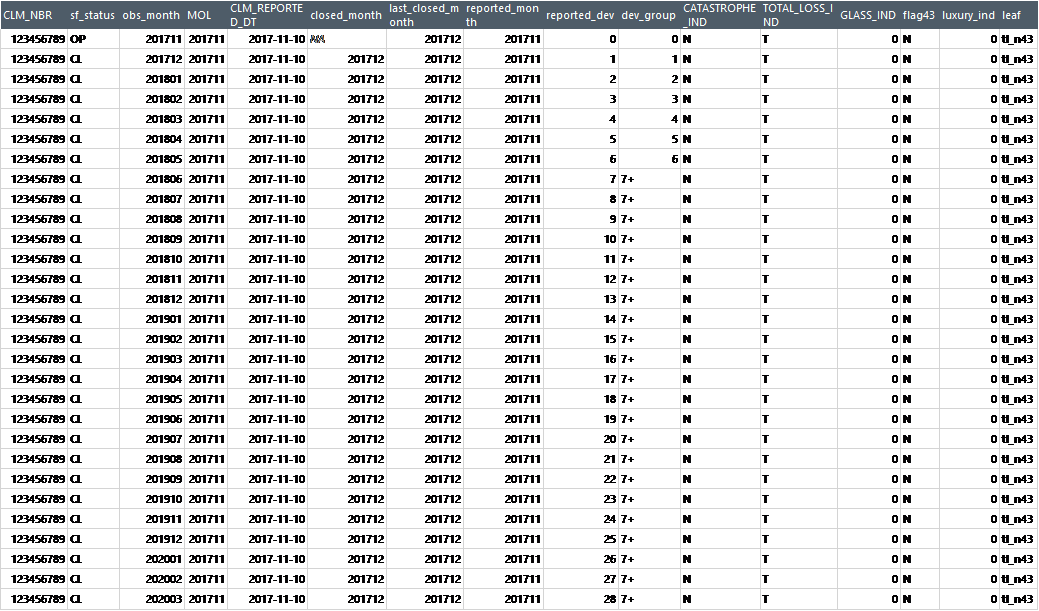
\includegraphics[scale=0.4]{Graphiques/sample_1} 
			\renewcommand{\figurename}{Figure}
			\caption{Sample from database}\label{Fig_sample_1}
		\end{center}
	\end{figure}
	
	In figure \ref{Fig_sample_2}, we have for each month of observation the amounts paid for the loss and alea.\\
	\texttt{AUTO\_LTD\_NET\_LOSS\_PAID\_AMT} is the paid amount known at the observation month. Any type of recovery can decrease the paid amount. \texttt{AUTO\_LTD\_LOSS\_RES\_CHG\_AMT} and \texttt{AUTO\_LTD\_LOSS\_RES\_CHG\_AMT} are the case reserve amounts at a given observation month. \texttt{AUTO\_LTD\_LOSS\_INCURRED\_AMT} and \texttt{AUTO\_LTD\_ALAE\_INCURRED\_AMT}, represent the incurred at the given observation month. The variables \texttt{FINAL\_NET\_PAID\_AMT} and \texttt{FINAL\_ALAE\_AMT} are the final amounts we know today, they are also called the ultimate amount for that claim. \texttt{AvgTypicalValue} (\texttt{ACV}) is an estimate of the market value of the accident vehicle. \texttt{TotalGAV} (\texttt{GAV}) is the gross appraisal value, which is the garage cost estimate to repair the vehicle. \texttt{IBC\_PRICE} is the initial purchasing price of the vehicle.\\
	\begin{figure}[H]
		\begin{center}
			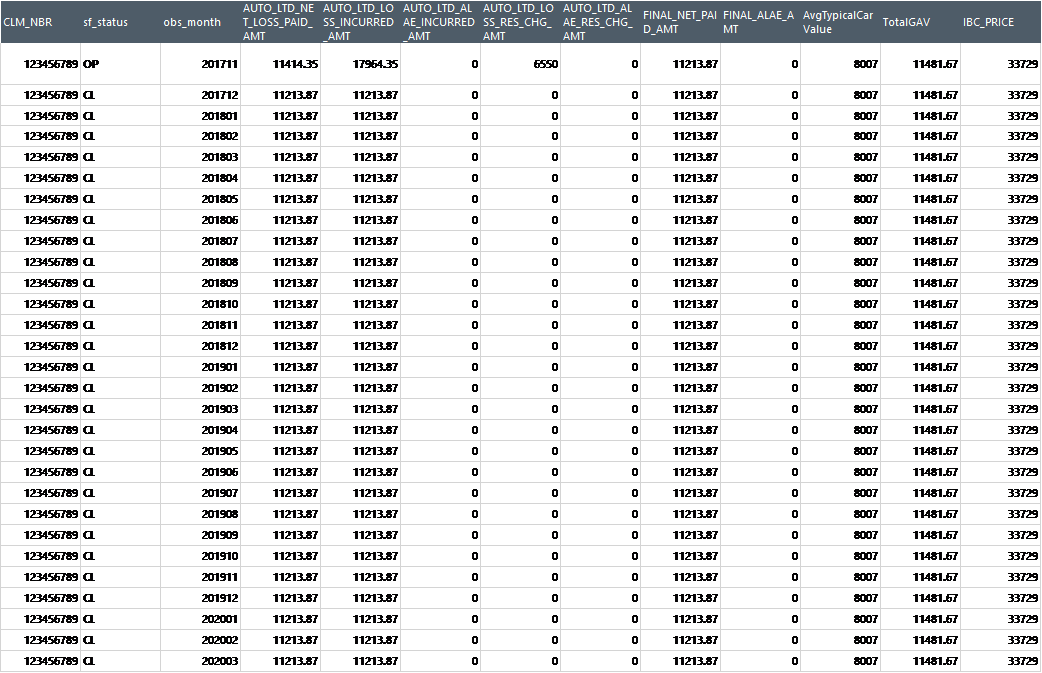
\includegraphics[scale=0.4]{Graphiques/sample_2} 
			\renewcommand{\figurename}{Figure}
			\caption{Severity sample from database}\label{Fig_sample_2}
		\end{center}
	\end{figure}

	Already with this single extract we can get a small understanding of our data. Specifically, we notice that the final paid amount, i.e. the ultimate, is close to \texttt{ACV} and \texttt{GAV} amount. This might indicate that the \texttt{ACV} and \texttt{GAV} are good predictors for our model. Consequently, we want to identify the dependence structure between the ultimate amount and the \texttt{ACV} or \texttt{GAV}. \\
	
	\subsection{Dependence structure}
	\cite{embrechts2001modelling}  show how copulas are used for modelling dependence between random variables. Even thou we do  not plan to model de dependence structure itself, we will use the copula to visualize the dependence. Since we are interested in more than only linear dependence, we will use Kendall’s tau as dependence measure. The definition of Kendall’s tau for a random vector pair $(X,Y)$ is given as
	
	$$ \tau(X,Y) = \Pr( (X - \widetilde{X}) (Y - \widetilde{Y}) > 0 ) - \Pr( (X - \widetilde{X}) (Y - \widetilde{Y}) < 0 )$$
	, where $(\widetilde{X},\widetilde{Y})$ is an independent copy of $(X,Y)$.\\
	
	It is the probability of concordance minus the probability of discordance. Concordance measures how X and Y move in the same direction relative to their independent copy. Discordance measures how X and Y move in opposite direction relative to their independent copy. It also can be interpreted as the correlation coefficient between the quantiles of X and Y, which have a relationship defined by a copula. Kendall’s tau has a value between -1 and 1. -1 indicates perfect negative dependence, also called countermonotonic, while 1 indicates perfect positive dependence, comonotonic. If Kendall’s tau is close to 0, the pairs are likely independent.\\
	A copula is a cumulative distribution function of a multivariate uniformed distribution. The copula of two independent uniform distribution $U_1 \sim U(0,1)$ and $U_2 \sim U(0,1)$, is defined as
	$$C(u_1,u_2) = u_1 \times u_2$$.
	
	A copula can be visualized by plotting pairs of quantiles of the uniform distributions. For the bivariate independent copula, the pairs are even distributed on the graph. Kendall’s tau should be close to 0 since it measures the correlation coefficient of these pairs. \\
	Before we can plot the ultimate and the \texttt{ACV/GAV}, we need to find their empirical quantile values between 0 and 1. We rank the values according to their relative size and divide each rank by the total number of observations. In addition, we will only use a sample of 10000 pairs, because we would have to many data points on the graph. We also use one single pair per claim number. Furthermore, we group the data into age since reported date categories. \\
	Starting with Quebec, figures \ref{Fig_copula_qc_rep} to \ref{Fig_copula_qc_tl} shows the copulas for each age grouping. On the x-axis we plot the quantiles of the ultimate amount (paid loss + alae) and on the y-axis we can see the quantiles of the\texttt{GAV}or \texttt{ACV}. We use the\texttt{GAV}for claims with repairable vehicles and the \texttt{ACV} for claims with vehicles that are total loss. On figure XXX we can observe the relationship between the ultimate and \texttt{GAV}. The relationship seems strong especially for younger claims (> 0.7). Note that Kendall’s tau decreases the older the claims become, indicating that older claims become more complex and incurred additional payments or recoveries which do not depend on the damage estimation. Figure XXX demonstrates a weaker dependence between the \texttt{ACV} and the ultimate. However, the dependence is still positive and not negligible. Further, it shows that the \texttt{ACV} might not always be a good estimation of the actual market value. The weaker dependence is therefore only caused by additional fees but also by intrinsic estimation error of the actual market value of the vehicle. 
	
	\begin{figure}[H]
		\begin{center}
			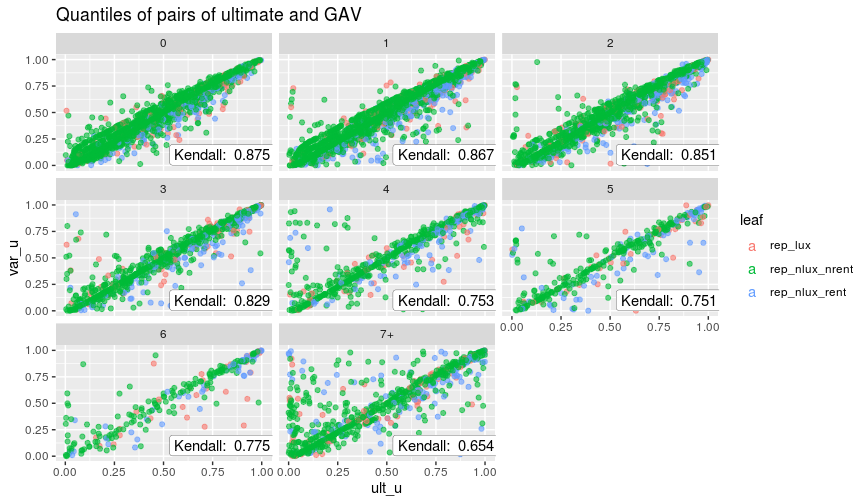
\includegraphics[scale=0.4]{Graphiques/qc_rep} 
			\renewcommand{\figurename}{Figure}
			\caption{Quantiles pairs for Quebec repairable claims. x-axis is the ultimate quantiles and y-axis the \texttt{GAV} quantiles}\label{Fig_copula_qc_rep}
		\end{center}
	\end{figure}

	\begin{figure}[H]
		\begin{center}
			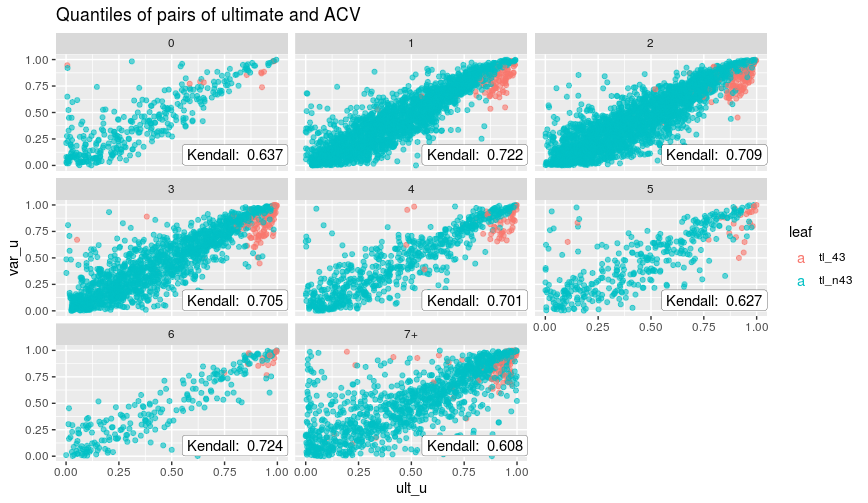
\includegraphics[scale=0.4]{Graphiques/qc_tl} 
			\renewcommand{\figurename}{Figure}
			\caption{Quantiles pairs for Quebec total loss claims. x-axis is the ultimate quantiles and y-axis the \texttt{ACV} quantiles}\label{Fig_copula_qc_tl}
		\end{center}
	\end{figure}

	For Ontario figure\ref{Fig_copula_on_rep} to \ref{Fig_copula_on_tl} should similar pattern than for Quebec. However, since we have two different line of businesses PHYSDAM and LIPD, it is interesting to observe the difference in pattern. LIPD tends to be more on the lower half of the diagonal. Third party liabilities seem to incur higher losses than the \texttt{GAV} would suggest and that it incurs more additional fees. 
	
		\begin{figure}[H]
		\begin{center}
			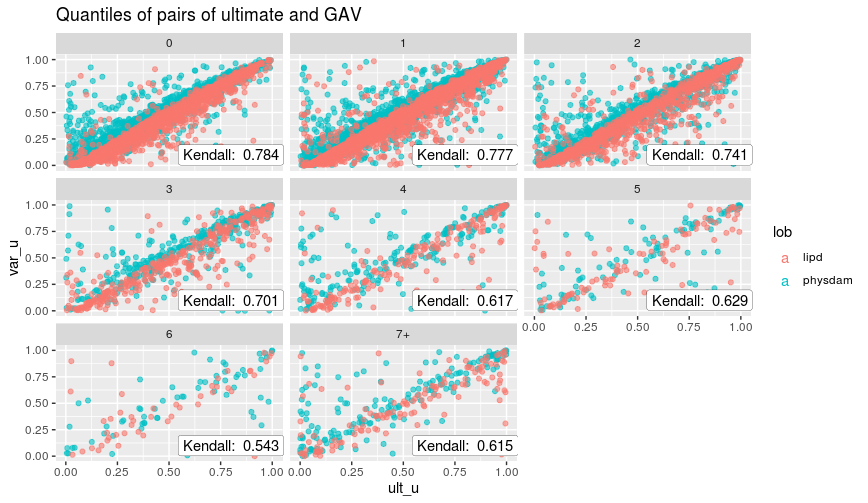
\includegraphics[scale=0.4]{Graphiques/on_rep} 
			\renewcommand{\figurename}{Figure}
			\caption{Quantiles pairs for Ontario repairable claims. x-axis is the ultimate quantiles and y-axis the \texttt{GAV} quantiles}\label{Fig_copula_on_rep}
		\end{center}
	\end{figure}
	
	\begin{figure}[H]
		\begin{center}
			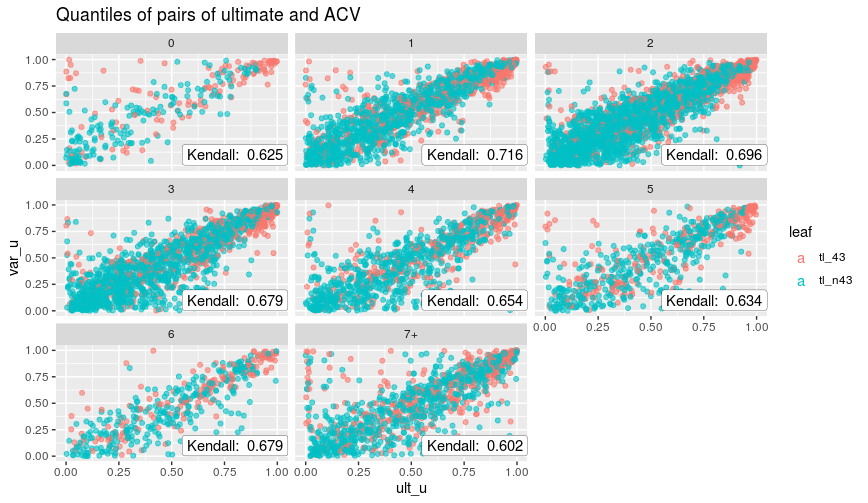
\includegraphics[scale=0.4]{Graphiques/on_tl} 
			\renewcommand{\figurename}{Figure}
			\caption{Quantiles pairs for Ontario total loss claims. x-axis is the ultimate quantiles and y-axis the \texttt{ACV} quantiles}\label{Fig_copula_on_tl}
		\end{center}
	\end{figure}
	
	Alberta shown in figure \ref{Fig_copula_ab_rep} to \ref{Fig_copula_ab_tl} has an interesting patterns. Again, we see weaker dependence for older claims. Albeit, there is a descriptive force which seem to strongly impact the dependence structure and leads to more claims with very low ultimate compared to the \texttt{GAV} or \texttt{ACV}. We identified this disruptive force as subrogation and recoveries. Subrogation is a slow process at which the insurance company can recover paid losses, if the insured was not responsible for the accident. This mean that if Intact paid the entire loss, they might be able to recover a part or the entire loss with a lawsuit. 
	
	\begin{figure}[H]
		\begin{center}
			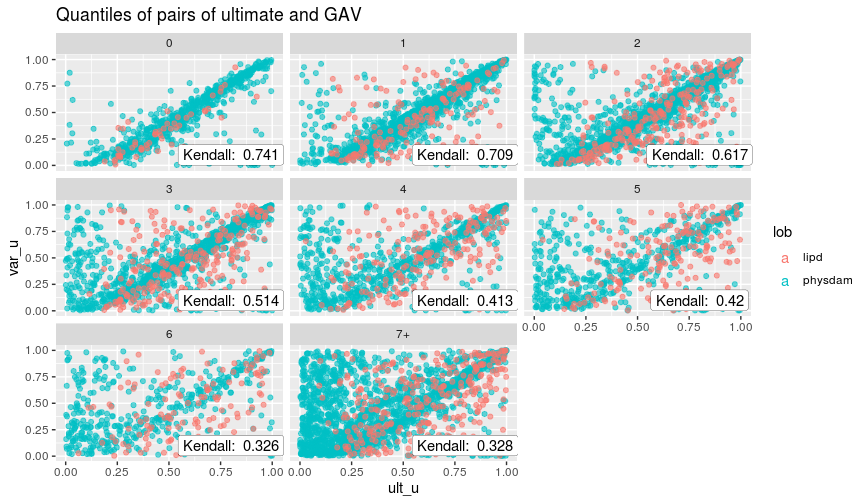
\includegraphics[scale=0.4]{Graphiques/ab_rep} 
			\renewcommand{\figurename}{Figure}
			\caption{Quantiles pairs for Alberta repairable claims. x-axis is the ultimate quantiles and y-axis the \texttt{GAV} quantiles}\label{Fig_copula_ab_rep}
		\end{center}
	\end{figure}
	
	\begin{figure}[H]
		\begin{center}
			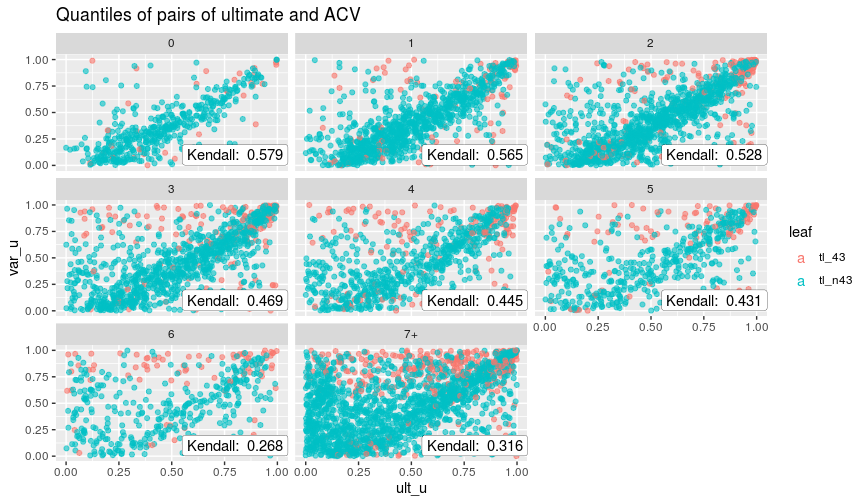
\includegraphics[scale=0.4]{Graphiques/ab_tl} 
			\renewcommand{\figurename}{Figure}
			\caption{Quantiles pairs for Alberta total loss claims. x-axis is the ultimate quantiles and y-axis the \texttt{ACV} quantiles}\label{Fig_copula_ab_tl}
		\end{center}
	\end{figure}

	The data indicates that it can take more than a year until the subrogation process is finished. Consequently, a proportion of claims in Alberta need much longer to fully develop to the ultimate which might even fall to 0 or negative. This can be problematic, since we are often unable to predict if the claim falls into the subrogation category or not. We can not filter out these claims, because for a given observation month, we do not know which claims a affected. We can partly mitigate this issue by aggregating the data and using averages. We can expect higher volatility in our model for Alberta. 
	All of these copulas also indicate a slightly stronger dependence for large/extreme values. 
	
	\subsection{Trend analysis}
	
	In our model we do not want to estimate the ultimate on a claim by claim basis, so we will aggregate the data. When aggregation data is important to verify the trends in data. If we use the \texttt{GAV} and the \texttt{ACV} as a predictor for the ultimate, we should verify that mean growth rates are similar. For each observation month we will calculate the mean ultimate and the mean \texttt{GAV}/\texttt{ACV} of open claims. Then, we will compare their monthly growth rates.  We could also do the same per month of loss, however, we want to analyse the underlying distribution of what we are trying to predict. Our model will predict the ultimate based on observation month data. Each observation month will contain a proportion of claims with different month of loss. While using aggregation per observation month, we have to be aware of possible fluctuations related to different number of claims and different mixtures of month of loss.\\
	When looking at figure \ref{Fig_QC_growth}, we can observe that in Quebec the average ultimate grows faster than the average \texttt{GAV}/ \texttt{ACV}. Using the\texttt{GAV}and \texttt{ACV} as predictor might tend to underestimate the ultimate if we use past averages. 
	
	\begin{figure}[H]
		\begin{center}
			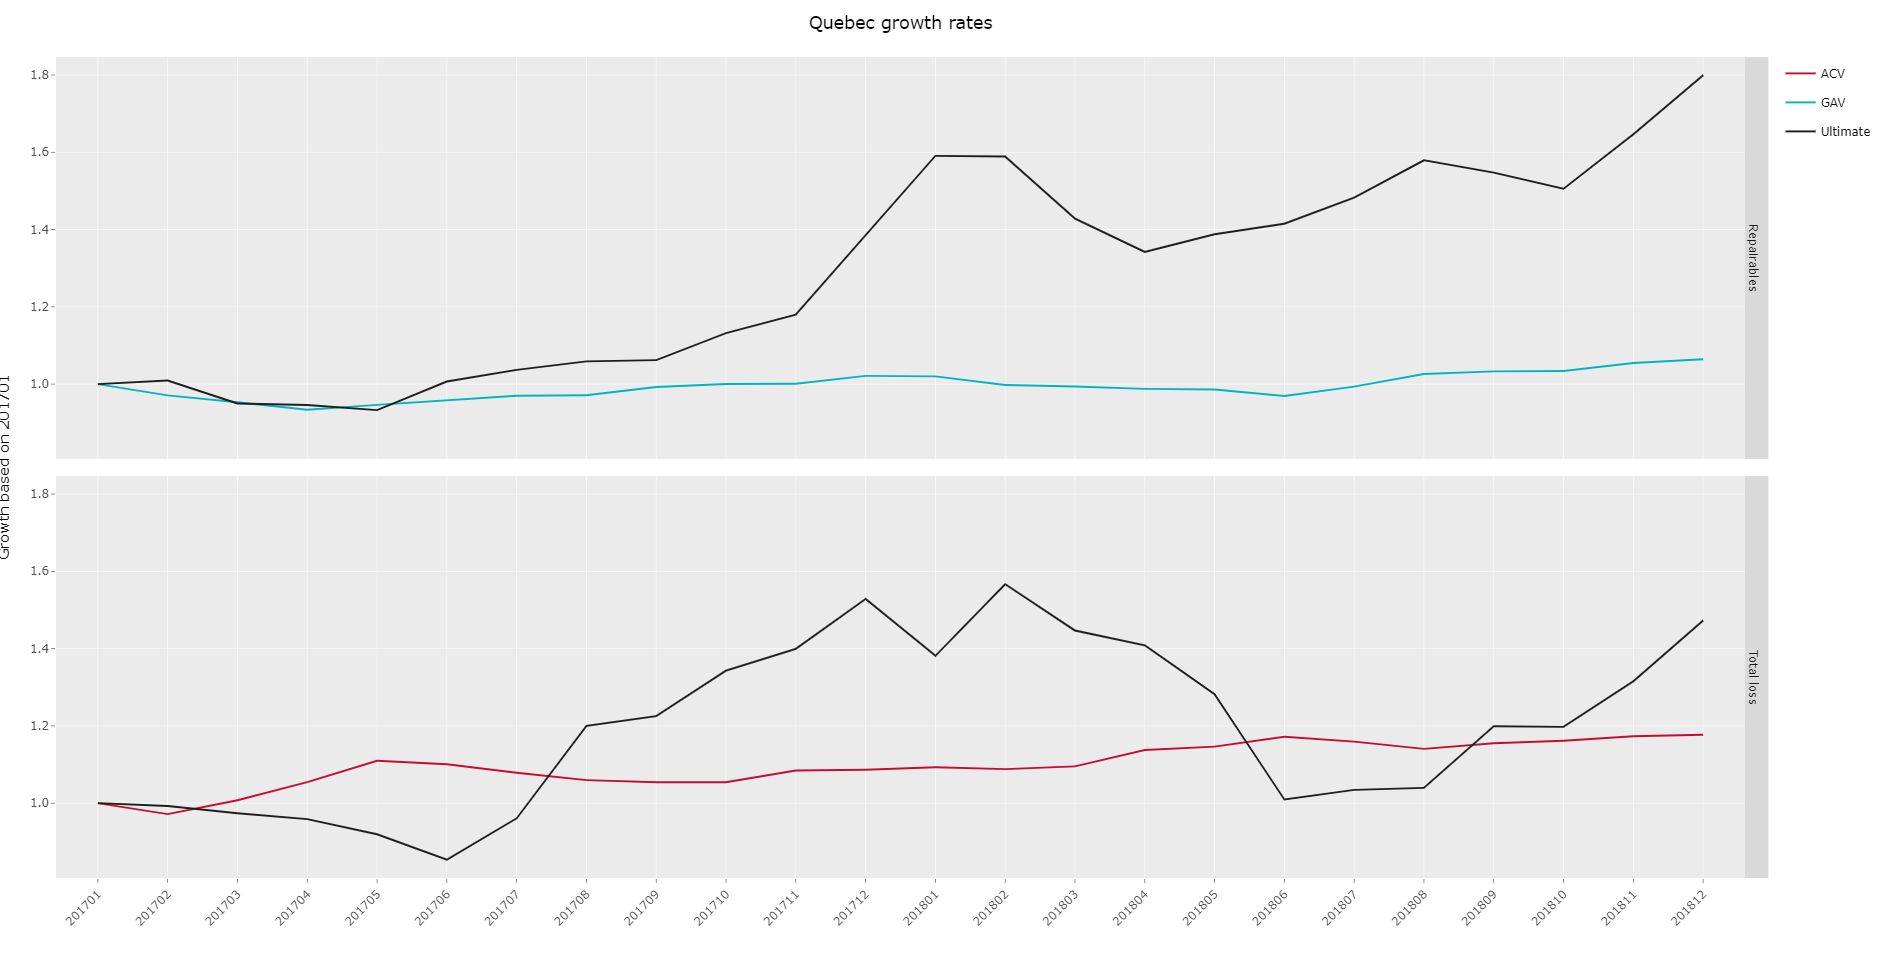
\includegraphics[scale=0.2]{Graphiques/QC_growth} 
			\renewcommand{\figurename}{Figure}
			\caption{Quebec ultimate and \texttt{GAV/ACV} growth relative to January 2017 (= 1)}\label{Fig_QC_growth}
		\end{center}
	\end{figure}

	In Ontario figure \ref{Fig_ON_growth}, the opposite seems to happen for total loss claims but not for repairable. Thus, we might tend to overestimate total loss claims ultimate.
	\begin{figure}[H]
		\begin{center}
			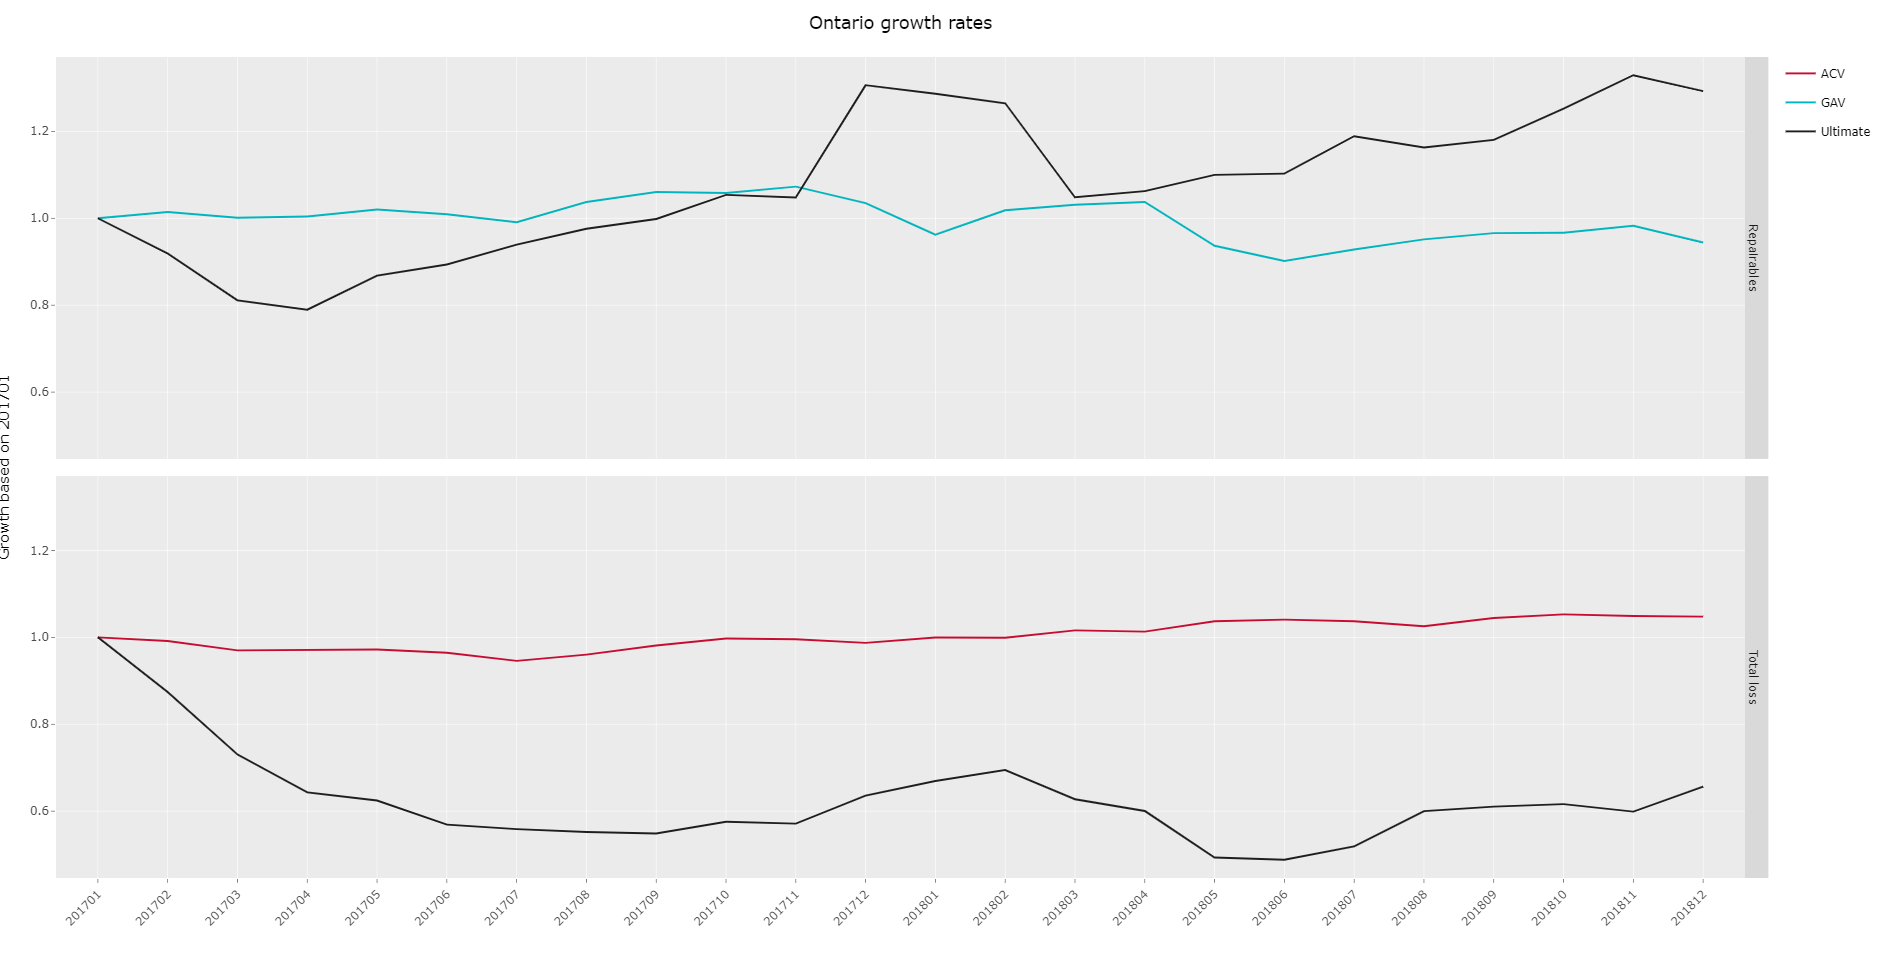
\includegraphics[scale=0.2]{Graphiques/ON_growth} 
			\renewcommand{\figurename}{Figure}
			\caption{Ontario ultimate and \texttt{GAV/ACV} growth relative to January 2017 (= 1)}\label{Fig_ON_growth}
		\end{center}
	\end{figure}
	On figure \ref{Fig_AB_growth}, Alberta has a similar but reversed pattern. Total loss claims ultimate growth fluctuates around the 1 value. While for repairables, growth rates for the ultimate are lower than for the \texttt{GAV}.  
	\begin{figure}[H]
		\begin{center}
			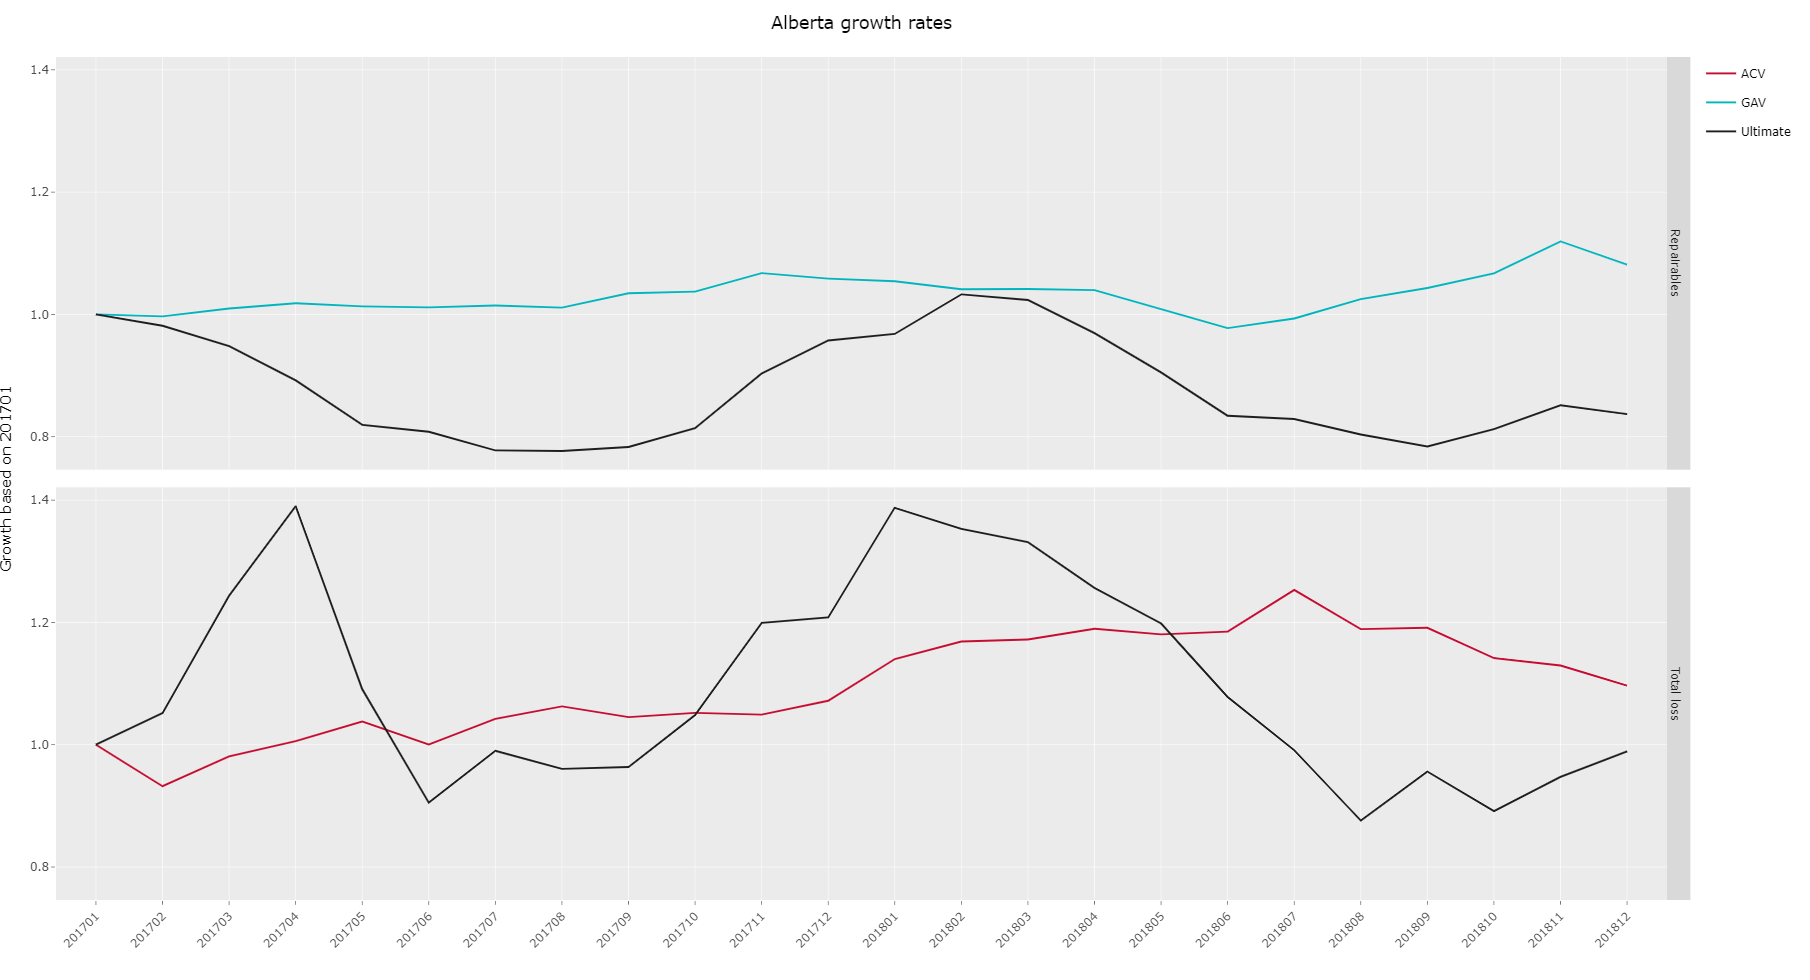
\includegraphics[scale=0.2]{Graphiques/AB_growth} 
			\renewcommand{\figurename}{Figure}
			\caption{Alberta ultimate and \texttt{GAV/ACV} growth relative to January 2017 (= 1)}\label{Fig_AB_growth}
		\end{center}
	\end{figure}
	
	CONFIDENTIEL???
	Furthermore, the \texttt{GAV} and \texttt{ACV} might not capture the additional costs related to the claim. The ultimate allocated loss adjustment expense (ALAE) is often unrelated to the \texttt{GAV} or \texttt{ACV}. A larger proportion of ALAE can cause greater estimation error. Figure \ref{Fig_QC_ALAE_loss} shows the ALAE to loss ratio for Quebec. The average is around 0.0125. In Ontario, seen in figure \ref{Fig_ON_ALAE_loss}, the ALAE to loss ratio is similar to the Quebec, although after December 2017 there is clearly a spike which might cause prediction errors. Alberta in figure \ref{Fig_AB_ALAE_loss} show again an different pattern than the other 2 regions. While most ratios are lower than in Quebec and Ontario, le non-luxury  non-rental repairable vehicles show proportionally larger ratios. 
	
	\begin{figure}[H]
		\begin{center}
			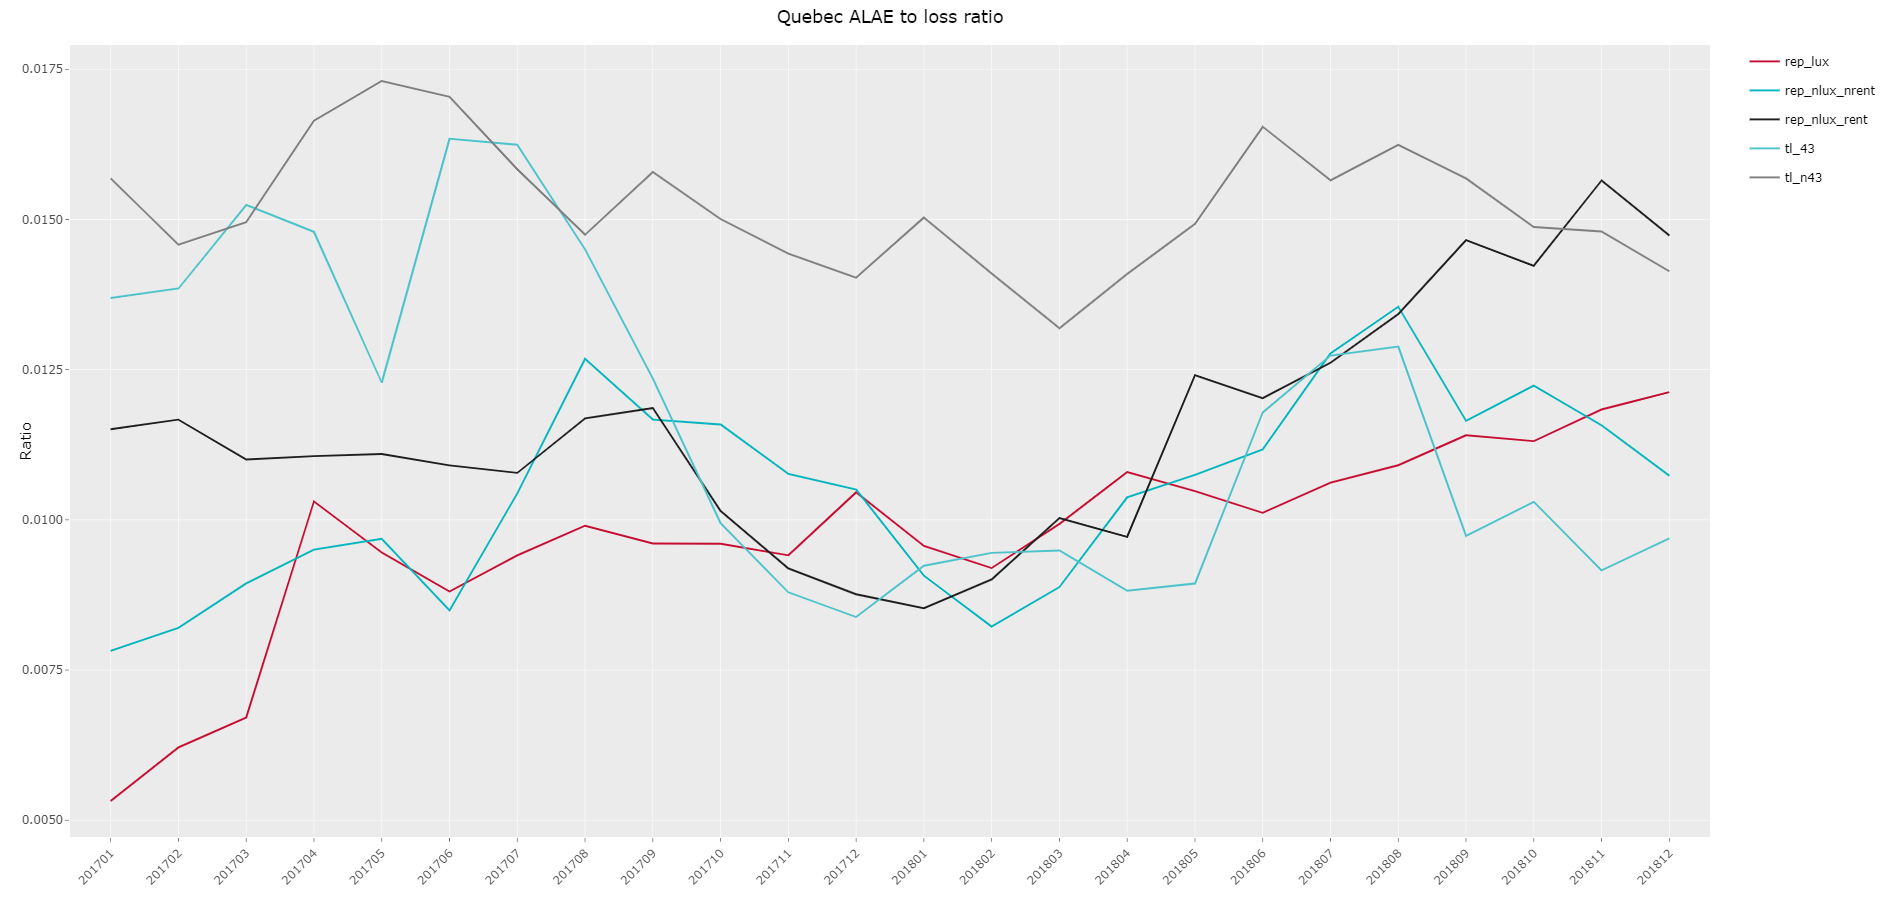
\includegraphics[scale=0.2]{Graphiques/QC_ALAE_loss} 
			\renewcommand{\figurename}{Figure}
			\caption{Quebec ALAE to loss ratio per \texttt{leaf}}\label{Fig_QC_ALAE_loss}
		\end{center}
	\end{figure}

	\begin{figure}[H]
		\begin{center}
				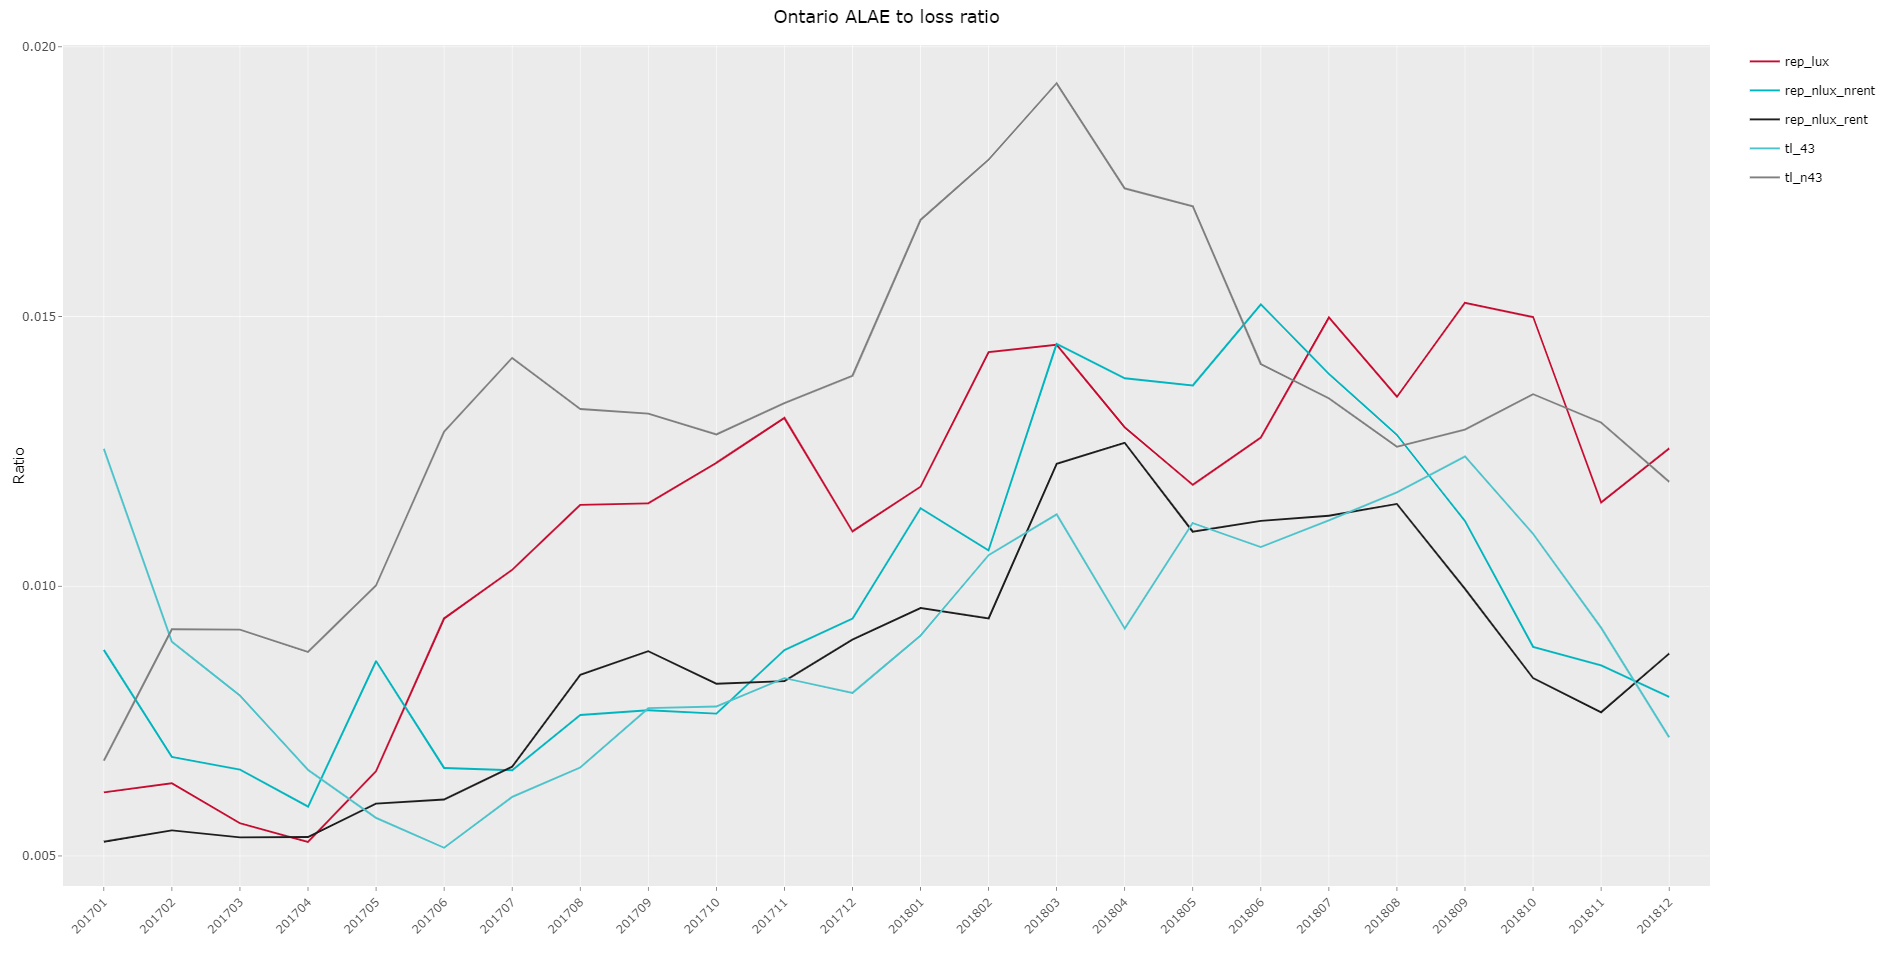
\includegraphics[scale=0.2]{Graphiques/ON_ALAE_loss} 
			\renewcommand{\figurename}{Figure}
			\caption{Ontario ALAE to loss ratio per \texttt{leaf}}\label{Fig_ON_ALAE_loss}
		\end{center}
	\end{figure}
	
	\begin{figure}[H]
		\begin{center}
				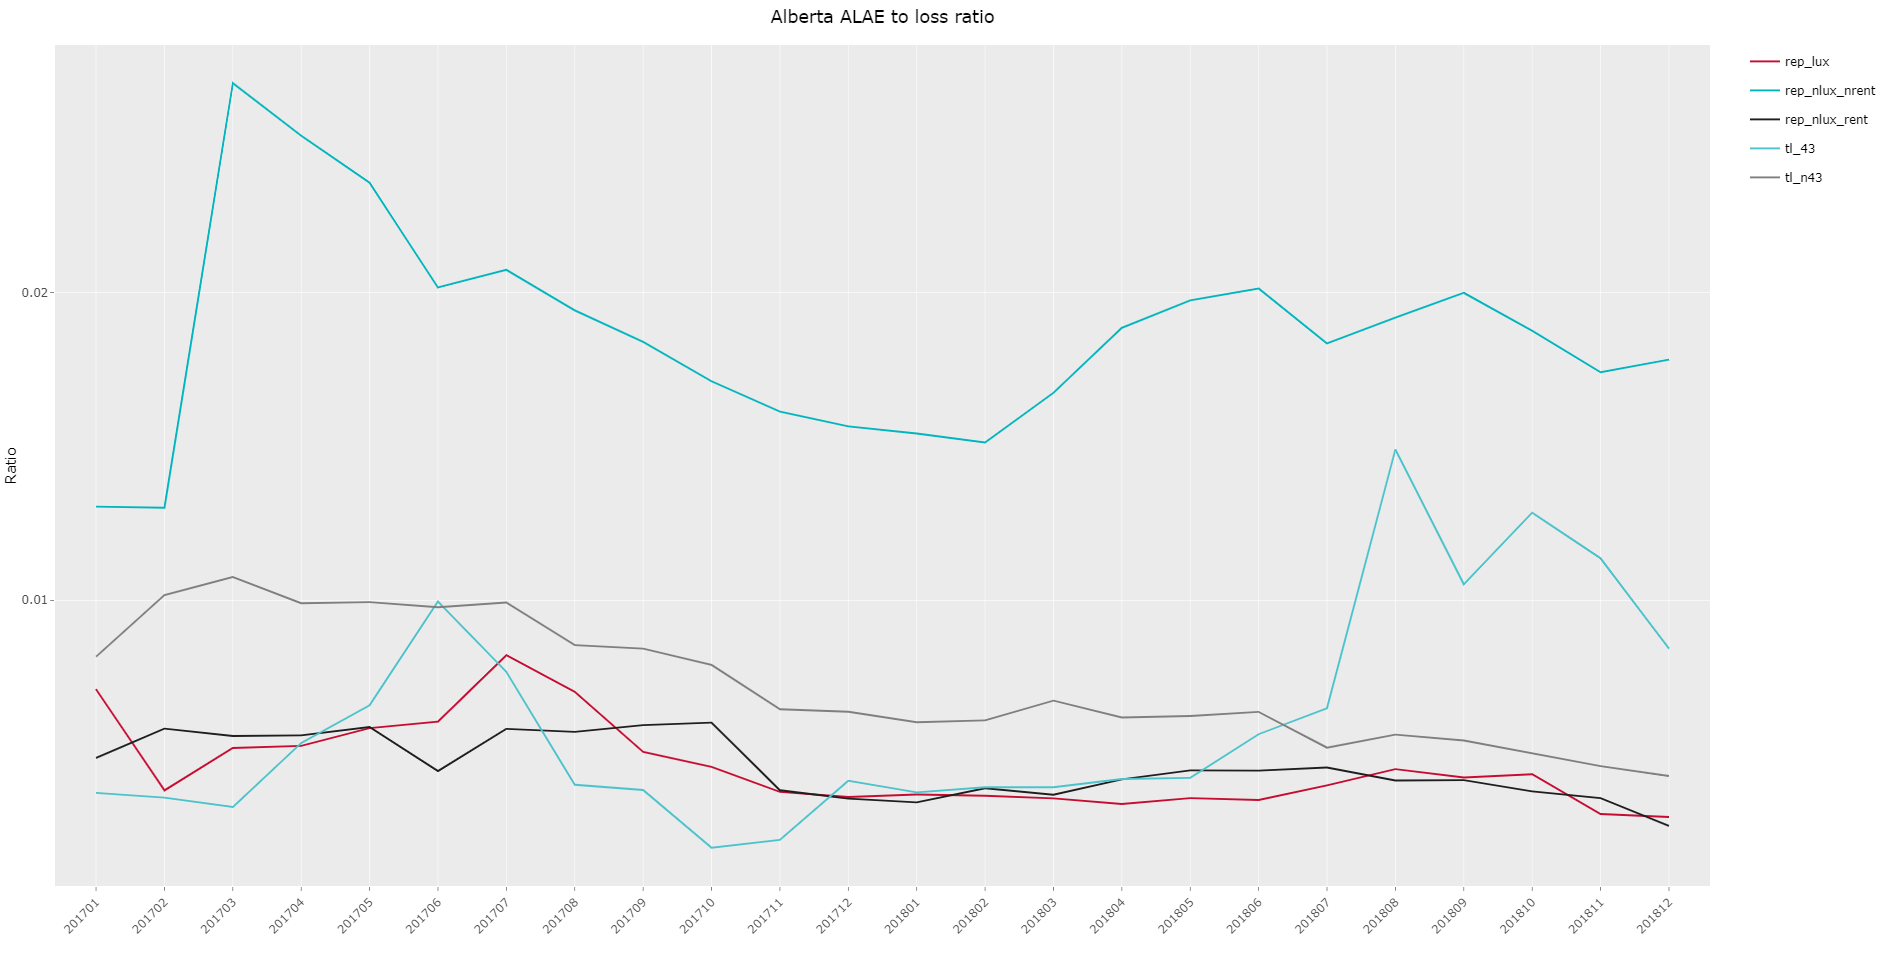
\includegraphics[scale=0.2]{Graphiques/AB_ALAE_loss} 
			\renewcommand{\figurename}{Figure}
			\caption{Alberta ALAE to loss ratio per \texttt{leaf}}\label{Fig_AB_ALAE_loss}
		\end{center}
	\end{figure}
	In order to better understand the impact of recovery on our data, figures \ref{Fig_QC_recovery_loss} to \ref{Fig_AB_recovery_loss} shows the recovery to ultimate ratio for all 3 regions. Quebec and Ontario both have a ratio below 0.17, while Alberta has ratios between 1 and 0.3. The discrepancy is very significant and has to be considered in our model.
		\begin{figure}[H]
		\begin{center}
			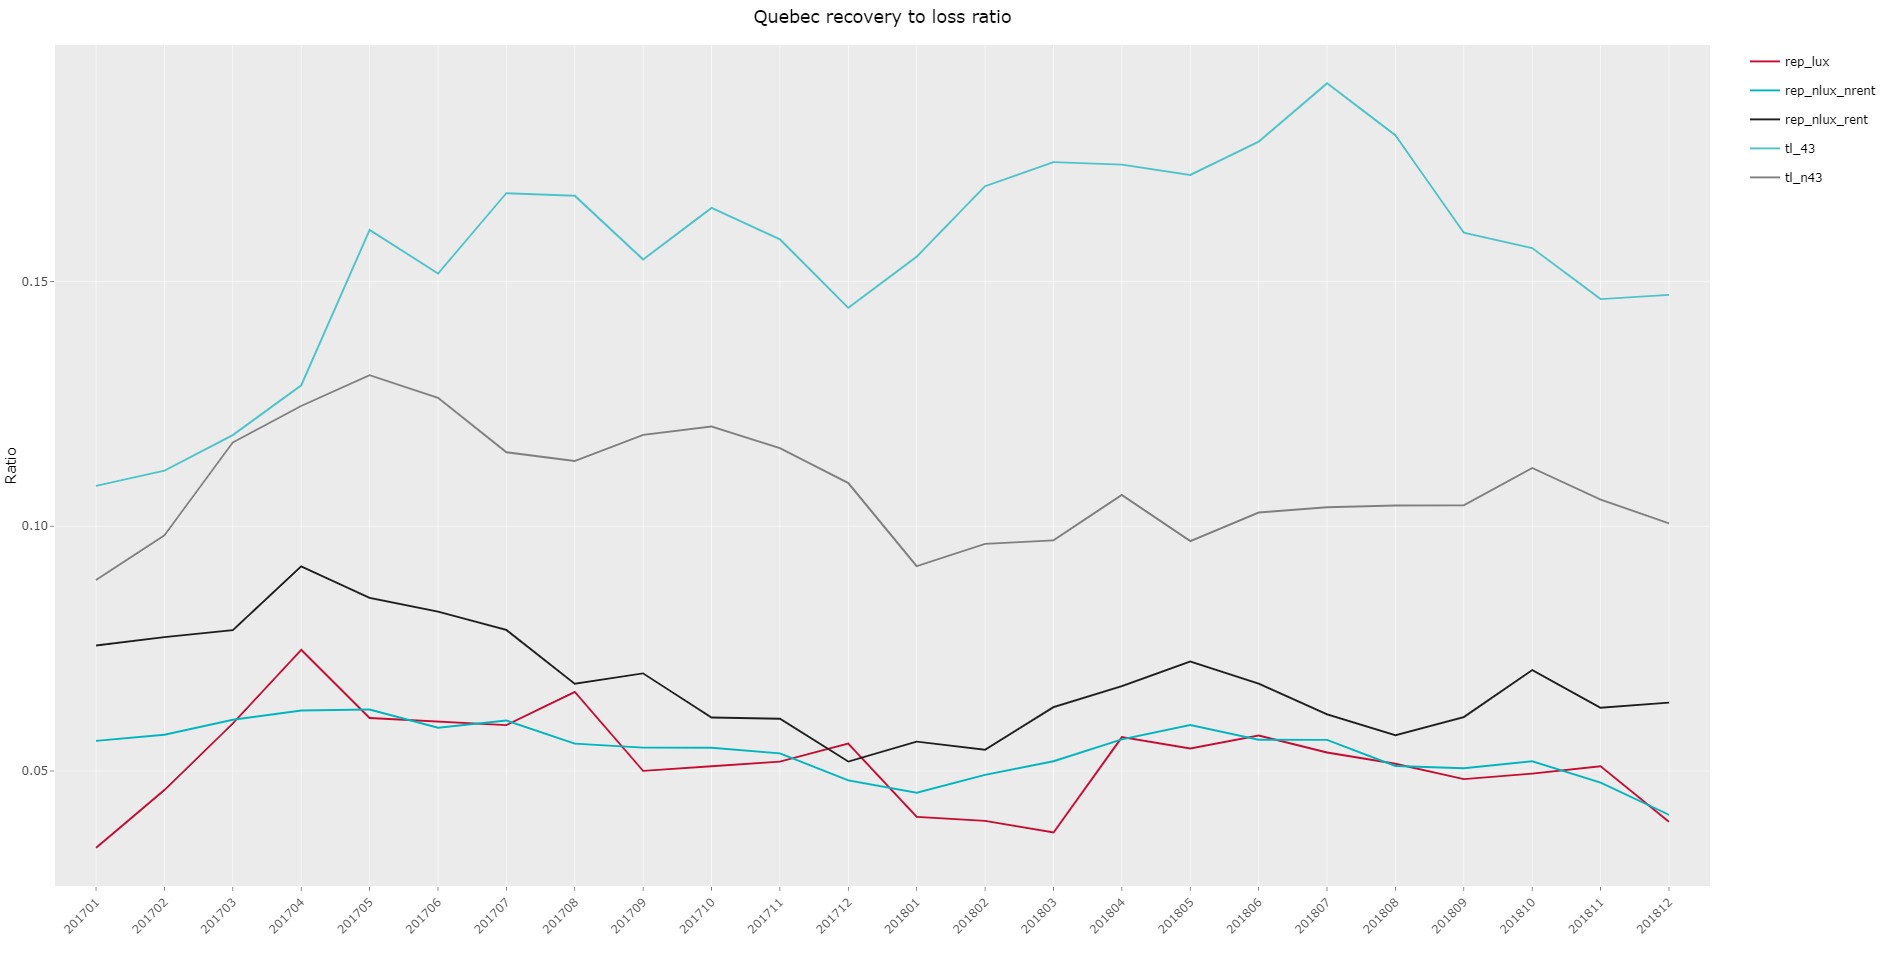
\includegraphics[scale=0.2]{Graphiques/QC_recovery_loss} 
			\renewcommand{\figurename}{Figure}
			\caption{Quebec recovery to loss ratio per \texttt{leaf}}\label{Fig_QC_recovery_loss}
		\end{center}
	\end{figure}
	
	\begin{figure}[H]
		\begin{center}
			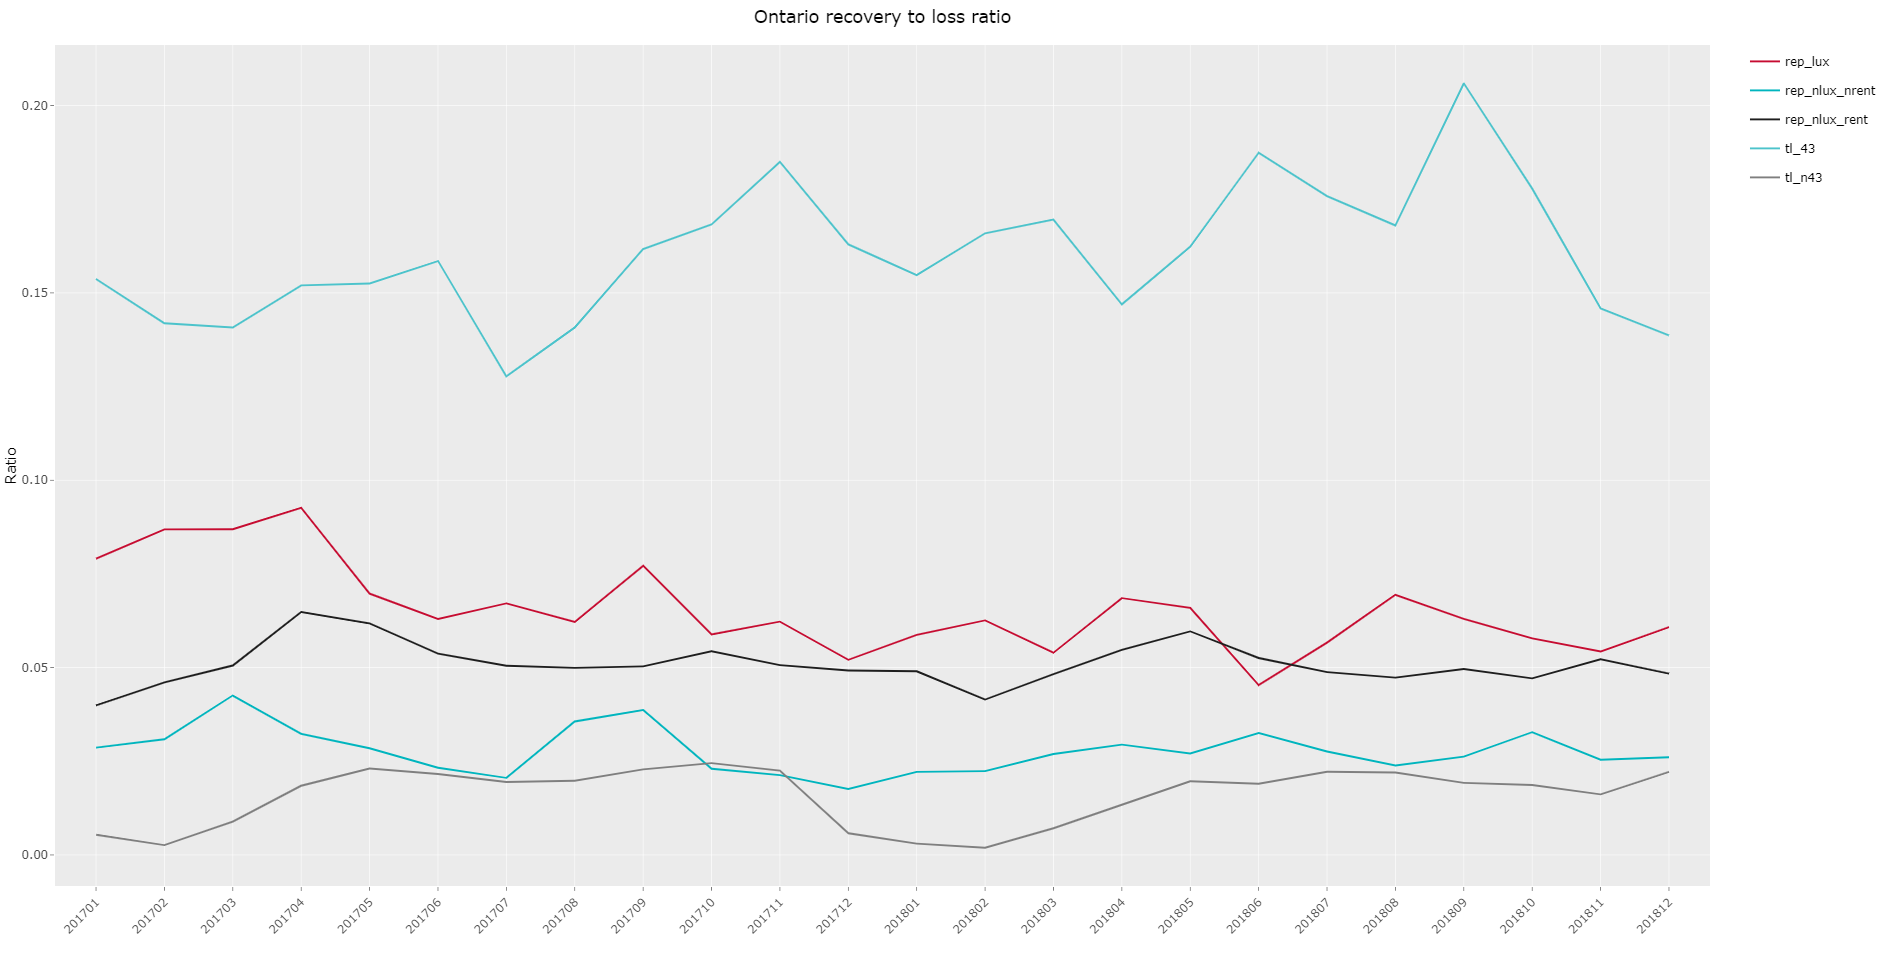
\includegraphics[scale=0.2]{Graphiques/ON_recovery_loss} 
			\renewcommand{\figurename}{Figure}
			\caption{Ontario recovery to loss ratio per \texttt{leaf}}\label{Fig_ON_recovery_loss}
		\end{center}
	\end{figure}
	
	\begin{figure}[H]
		\begin{center}
			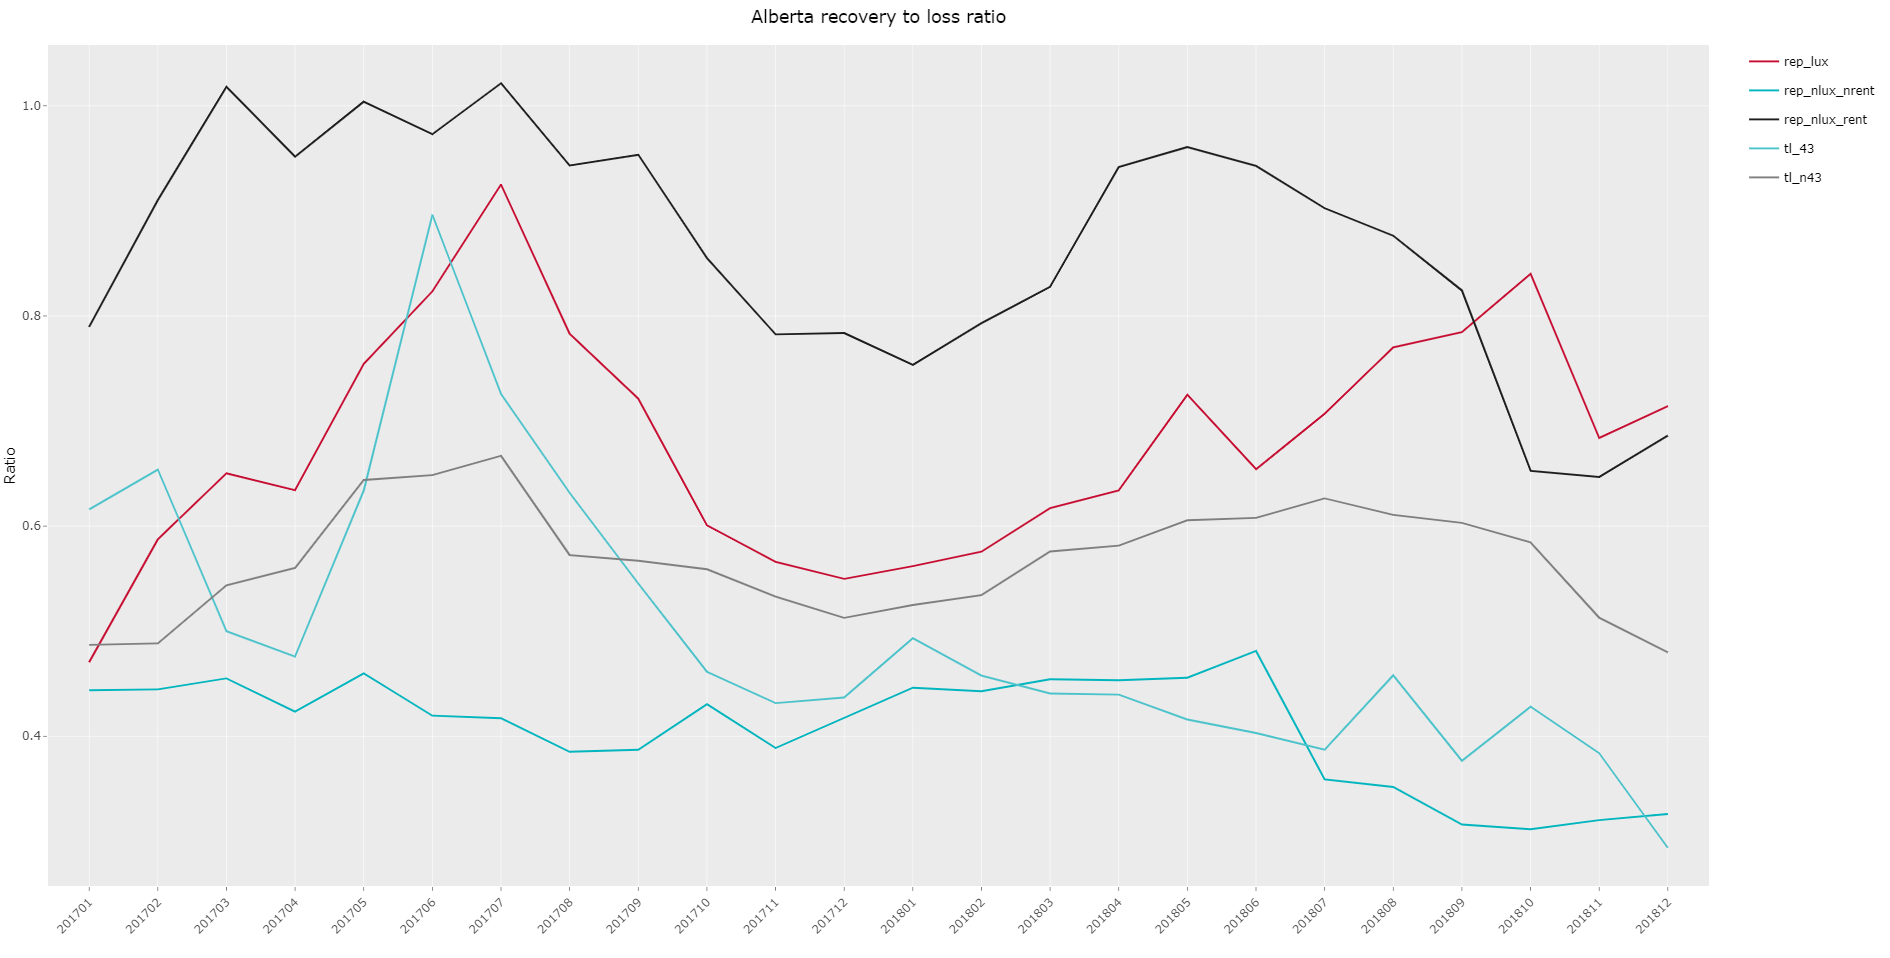
\includegraphics[scale=0.2]{Graphiques/AB_recovery_loss} 
			\renewcommand{\figurename}{Figure}
			\caption{Alberta recovery to loss ratio per \texttt{leaf}}\label{Fig_AB_recovery_loss}
		\end{center}
	\end{figure}
	
	Now that we have a better understanding of our data, we will discuss the model structure and methodology.
	
	 
	\section{Model methodologie}\label{Sect_Methodologie}
\subsection{Incurred but not reported}
	The task of the actuarial model is to predict the IBNR, the incurred but not reported claims. The IBNR can be divided into 3 distinct elements, which we defined as pure IBNR, IBNER and unpure IBNR. Pure IBNR are claims which are not reported at the observation date, meaning the insurer has no information on them. The insurer only knows that a claim happened. IBNER, incurred but not enough reported, are claims which have been reported and the insurer the information on the claims in their database. Unpure IBNR consist of claims which might reopen at any given time. This mean that a claim which closed in 2017 might reopen in 2018 or 2019. Unpure IBNR is a small proportion of the total IBNR, but still should be considered in the model. Figure XXX gives a visual representation of these categories. 
	\begin{figure}[H]
		\begin{center}
			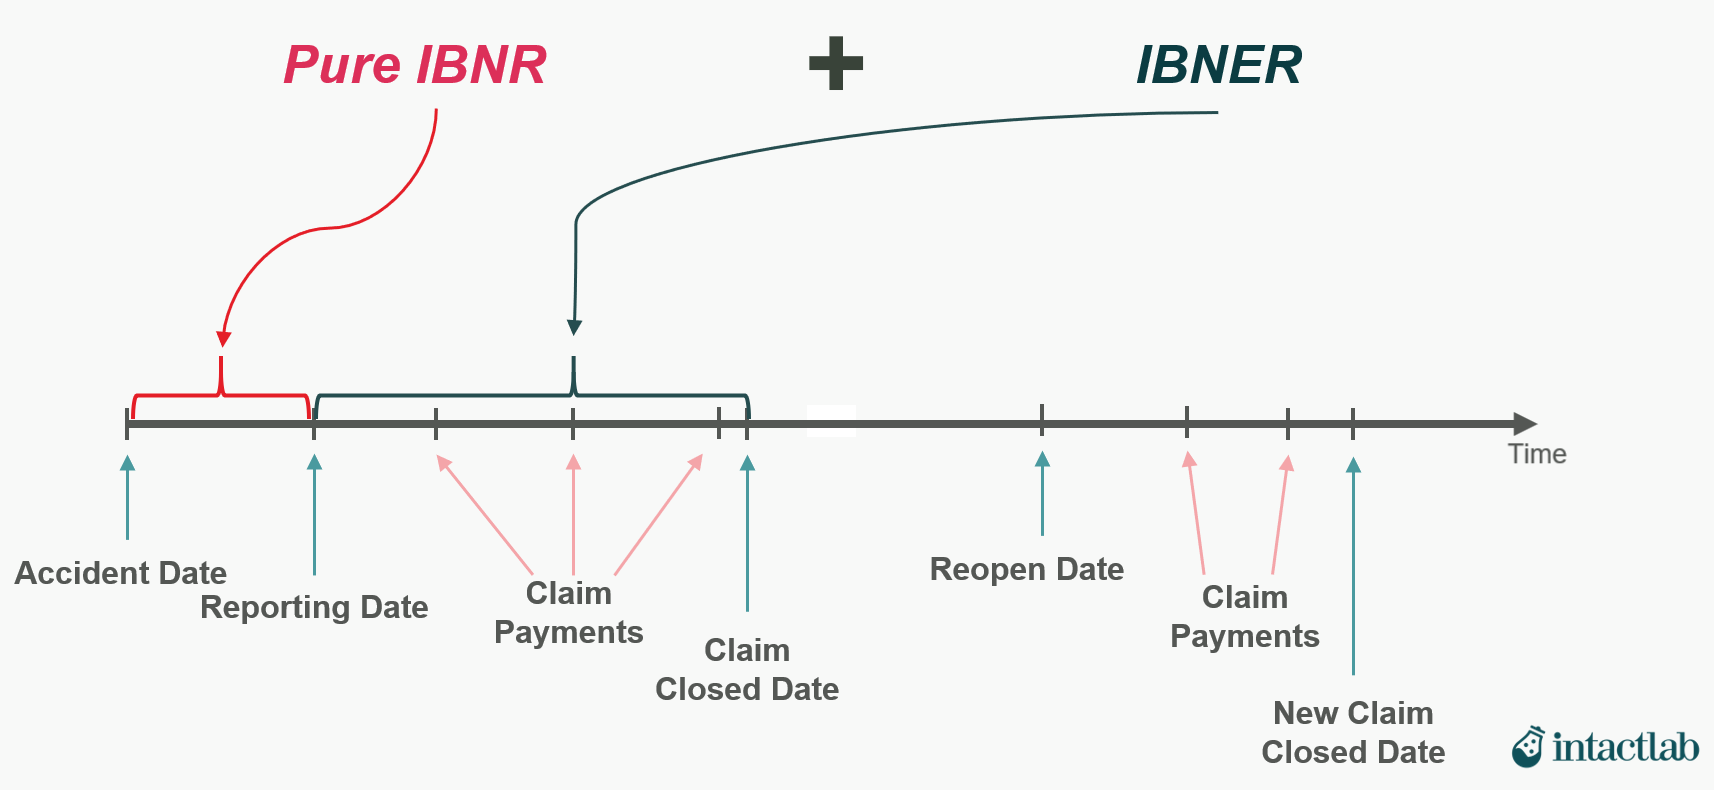
\includegraphics[scale=0.2]{Graphiques/IBNER_timeline} 
			\renewcommand{\figurename}{Figure}
			\caption{Timeline of a claim}\label{Fig_IBNER_timeline}
		\end{center}
	\end{figure}

\subsection{Hierarchical approach}
	The actuarial department uses a modified chain-ladder method for their model. We will try a more hierarchical approach, where we cluster our data in more homogeneous groups. First, we develop a model for each of the three IBNR types. Our team focuses on the IBNER part, while the pure and unpure IBNR models are still chain-ladder based and were developed by the actuarial department. For the IBNER model, we grouped the data according the following claims characteristics:  total loss, total loss without (\texttt{43}) replacement cost endorsement (\texttt{n43}), luxury repairable vehicles (\texttt{rep\_lux}), non luxury non rental repairable vehicles (\texttt{rep\_nlux\_nrent}) and non luxury rental repairable vehicles (\texttt{rep\_nlux\_rent}). We suppose that the frequency and severity distributions are very similar within these groups. Figure XXX gives an overview of the hierarchical approach.
	\begin{figure}[H]
		\begin{center}
			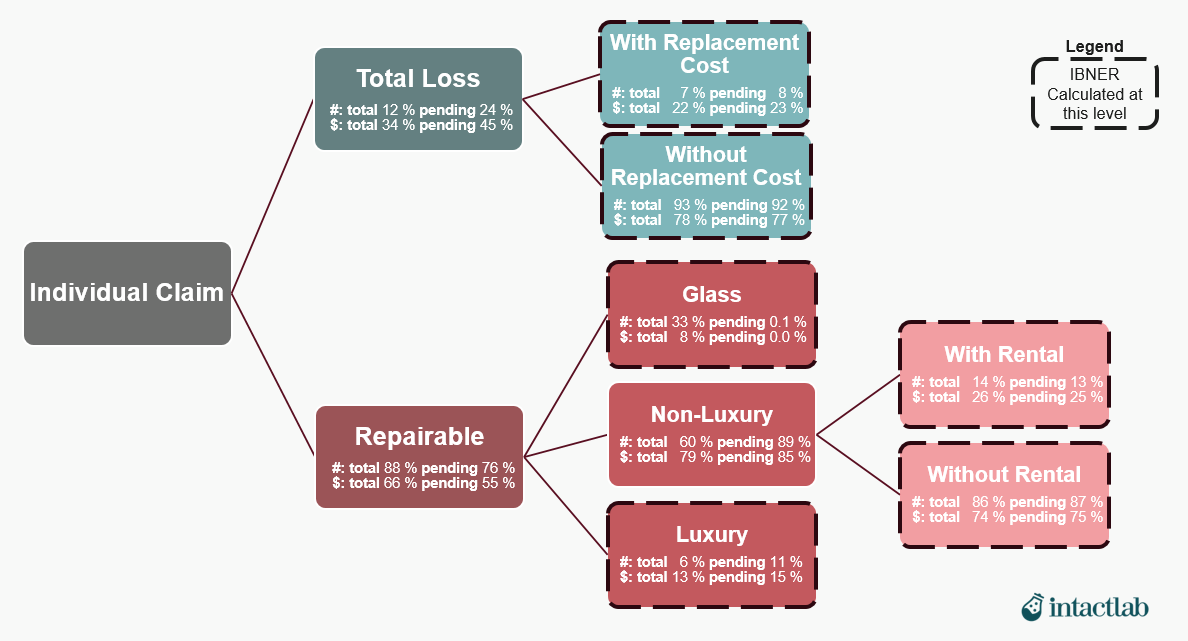
\includegraphics[scale=0.4]{Graphiques/Hier_model} 
			\renewcommand{\figurename}{Figure}
			\caption{Hierarchical model structure}\label{Fig_hier_model}
		\end{center}
	\end{figure}
 
\subsection{Key formulas}
	As mentioned in section ???, the ACV and GAV have strong predictive strength. We will use a basic formula to link the GAV/ACV with the ultimate and use historical observation on the pending (open) claims.

	 
	\begin{Definition}
		We define $\hat{L}_i$ as ultimate loss prediction for claims pending/open in period $i$ and $X_i$ as the predictor, in our case \texttt{GAV} or \texttt{ACV} used to predict period $i$. Their relationship is defined as
		$$\hat{L}_i = \hat{\Theta}_i \times X_i$$
		Where $\hat{\Theta}_i$ is the factor for time period $i$.
	\end{Definition}
	We need to calculate the factor $\hat{\Theta}_i$ with the available historical data. 
	\begin{Definition}
		We define $\widetilde{L}_{j,i}$ as total incurred for claims in time period $j$ as of $i$. $X_j$ is the predictor in time period $j$. Thus, the factor is defined as
		$$\hat{\theta}_i = \frac{\widetilde{L}_{j,i}}{X_j}$$
	\end{Definition}

	Note the difference between $\hat{L}_i$ and $\widetilde{L}_{j,i}$. The former is the ultimate we want to predict, so we do not know its value in observation month $i$. The latter is the total incurred for claims in period $j$ we know as of $i$. For illustration in the sample data of figure XXX and XXX, we want to calculate the factor $\hat{\theta}_{201804}$. We suppose we want to use open claim with $ \texttt{CLM\_NBR} = 123456789$ to calculate this factor, then 
	\begin{align*}
	\widetilde{L}_{201711, 201804} &= \texttt{AUTO\_LTD\_NET\_LOSS\_PAID\_AMT} + \texttt{AUTO\_LTD\_ALAE\_INCURRED\_AMT} \\
									& \ \ \	+ \texttt{AUTO\_LTD\_LOSS\_RES\_CHG\_AMT} \\
									&= 11213.87
	\end{align*}
	 as of $201804$ ($\texttt{obs\_month} = 201804$) and $X_j = \texttt{AvgTypicalCarValue} = 8007 $.
	As the example illustrated, the ultimate and the predictor are historical values which should be fully developed. It is necessary to have a least 5 to 12 months of development, so that the factors are stable enough. The difference in time between the moment we want to predict the pending and the historical data, $i - j$ is defined as the lag. How many historical observation month $j$ we use for the calculation is defined as period length. Figure XX shows a 5 months lag and 3 months period length. We want to predict the ultimate of the December 2018, $i = 201812$ pending (open) claims. We go back 5 months and use the historical claim data from open claims in May, June and July 2018, $j=201805, 201806, 201807$. 
	\begin{figure}[H]
		\begin{center}
			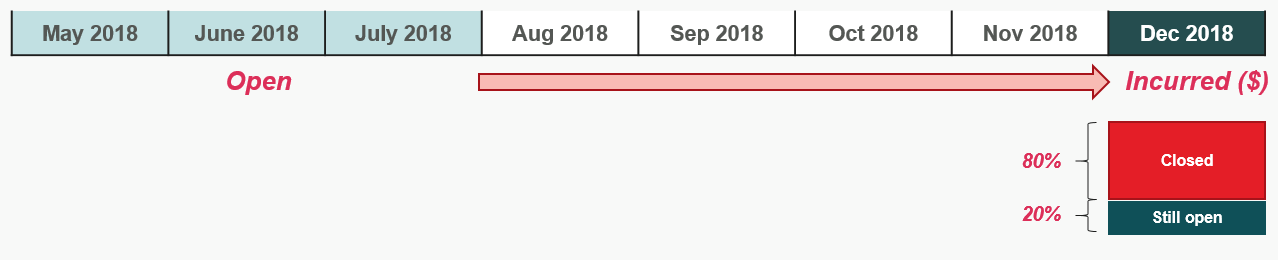
\includegraphics[scale=0.4]{Graphiques/lag_pl} 
			\renewcommand{\figurename}{Figure}
			\caption{Lag and period length visualization}\label{Fig_lag_pl}
		\end{center}
	\end{figure}
	This approach is similar to a lagged moving average model. We use the incurred as of December 2018 of claims open in May, June and July. Thus, the incurred had a minimum of 5 months to develop. Then, we divide this incurred by the aggregated GAV or ACV in May, June and July. We only keep the most recent data line for each claim, in other words we don’t have any duplicated per claim number. Figure XX gives a numerical example. 
	\begin{figure}[H]
		\begin{center}
			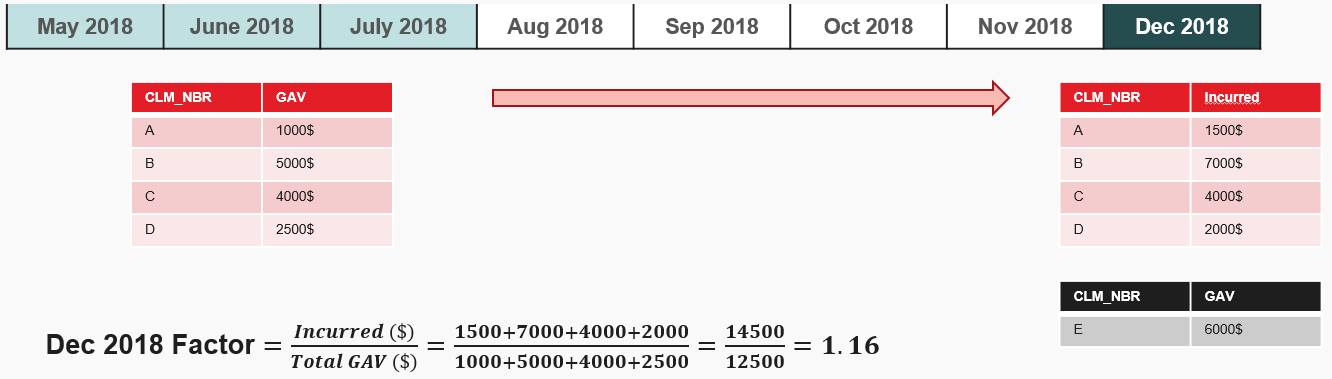
\includegraphics[scale=0.4]{Graphiques/factor_example} 
			\renewcommand{\figurename}{Figure}
			\caption{Factor calculation example}\label{Fig_factor_example}
		\end{center}
	\end{figure}
	Note that in figure \ref{Fig_lag_pl} the incurred is subdivided into open and closed claims, since it is possible that claims remain open even after 5 months. Therefore, we will calculate a claim number weighted average of closed and open factors. We get as final factor
	\begin{Definition}\label{Def_final_factor}
		$\hat{\Theta}_i$ is the final factor used for the prediction. $\hat{\theta}_{i,open}$ is the factor for claims that are still open during $i$ and  $\hat{\theta}_{i,closed}$ is the factor for claims that are closed during $i$. Furthermore, $n_{open}$ is the number of open claims in period $i$ and $n_{closed}$ is the number of closed claims in period $i$. Thus, we have
		$$\hat{\Theta}_i = n_{open} \hat{\theta}_{i,open} + n_{closed} \hat{\theta}_{i,closed}$$ 
	\end{Definition}
	
	We multiply this factor by the aggregated GAV or ACV of pending claims (December 2018 in our example) to get the ultimate amount.
	
	\begin{Definition}
		We define the $IBNER$ in period $i$ as
		$$IBNER_i = \hat{L}_i - I_i$$
		, where $I_i$ is the incurred payments and reserve for claims pending in period $i$.
	\end{Definition}
	Note that once claims are fully developed $L_i = I_i$, where $L_i$ is the real observed ultimate loss for claims open in period $i$. 
	The prediction results for the model will be discussed in section XX.
	
\subsection{Imputation methodology}
	It is important to note that no data is perfect. Our dataset contains a non negligible amount of missing GAV and ACV values. About 17\% of the claims have missing GAV or ACV, some regions and line of business are worse than others. Figure XX demonstrates how missing values are imputed. If we have missing values, we calculate the median of the existing values in the time window. We replace the missing values by the median and execute the factor calculations without any further readjustment. This method is not perfect and will be revised. For instance, in our example, we would overestimate the factor since we impute with a lower value.  
	\begin{figure}[H]
		\begin{center}
			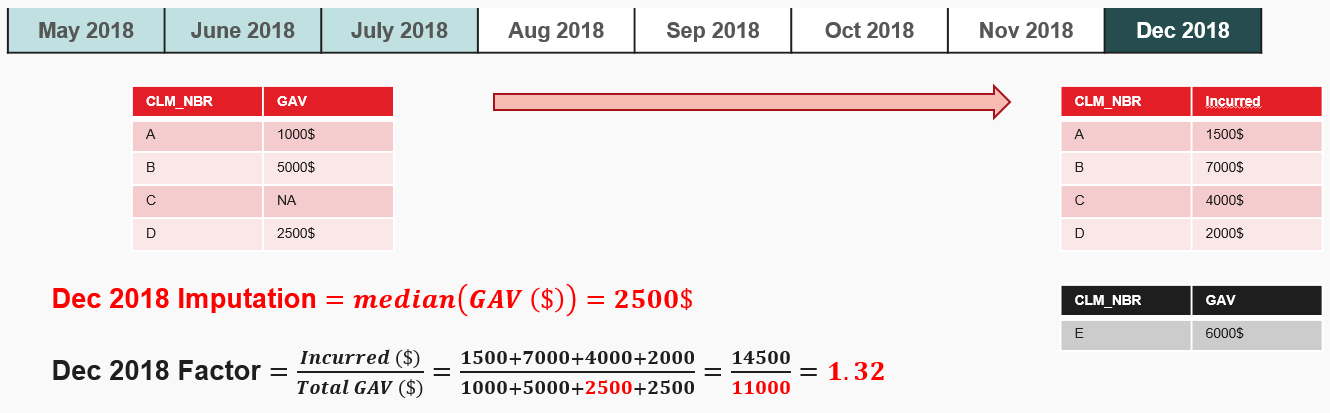
\includegraphics[scale=0.4]{Graphiques/imputation_example} 
			\renewcommand{\figurename}{Figure}
			\caption{Factor calculation example with missing values}\label{Fig_imputation_example}
		\end{center}
	\end{figure}

\subsection{Adjusting the lag and period length}
As we have noticed in the analysis of the data, Alberta clearly has different patterns than the other regions. Claims in Quebec and Ontario settle considerably faster (after 4-5 months) and recovery is less impactful. In Alberta having a lag of 5 is clearly insufficient, thus we will use a lag of 10. This gives the claims at least 10months to fully develop. In addition, a lag and period length that includes the 12th month, is beneficial if we have seasonal effects.
\subsection{Second model iteration: Historical pending but now closed claims}
After having used the first iteration of the model for January 2020. We noticed systematic error, constant over- or underestimations. This might be related to the open claims (after the lag) with are used to calculate the factors. Since open claims still have a case reserve the incurred used for the factor might be inflated, thus explaining overestimation. Indeed, the factor for open claims is always larger than the factor for closed. If we overestimate constantly, we attribute to much weight to still open claims. In the second iteration of the model we discard the weighted average and we only use the factor of closed claims. In short, based on definition \ref{Def_final_factor}, we have
$$\hat{\Theta}_i = \hat{\theta}_{i,closed}$$.
This also has the benefit that closed claims usually should not develop further and thus have less volatility in the calculation of the factors. The results will be discussed in section XXX.
\subsection{Third model iteration: Historical closed claims}
The final iteration of the model we will discuss in this report is based on the idea of the second iteration. We only want to use the factor of closed claims. However, in the second iteration we use the factor of closed claims of the lagged 3 month period, while in this iteration we want to increase the number of claims used in the calculations and add more recent claims. Consequently, instead of using the pending claims in a historical time window, we calculate factors for all claims that closed in the time window. This simply implies changing the filter on \texttt{sf\_status}. If we have use the previous example, we want to predict the pending claims in December 2018, we use all claims that closed between May and July for our factor calculations. Since the claims are closed it is unlikely that we have still open claims in December.

	\section{Results}\label{Sect_Results}
In this section we will analyse the results of all 3 model iterations. For the first two iterations we will show the prediction error on the ultimate for each \texttt{leaf} and province, while for the last iteration will will give the average monthly error. It should be notes that we only show the ultimate predictions for claims pending in 2017 and 2018, although we use the incurred as of March 2020. Pending claims in December 2018 had more than 14 months to develop to the ultimate. 
\subsection{First model iteration: Historical pending claims}
	\paragraph{Quebec:}
		For our first model, the average monthly prediction error is $957 757.84$, based on a total volume of about 100 million. Figure \ref{Fig_QC_current_er_by_month} show that the error has a light seasonal pattern. In winter we tend to slightly underestimate, while in most months we overestimate the ultimate loss. The seasonality is difficult to confirm, since we only have 2 years of fully credible data. The error does not seem to be all random and thus should be further investigated.
		\begin{figure}[H]
			\begin{center}
				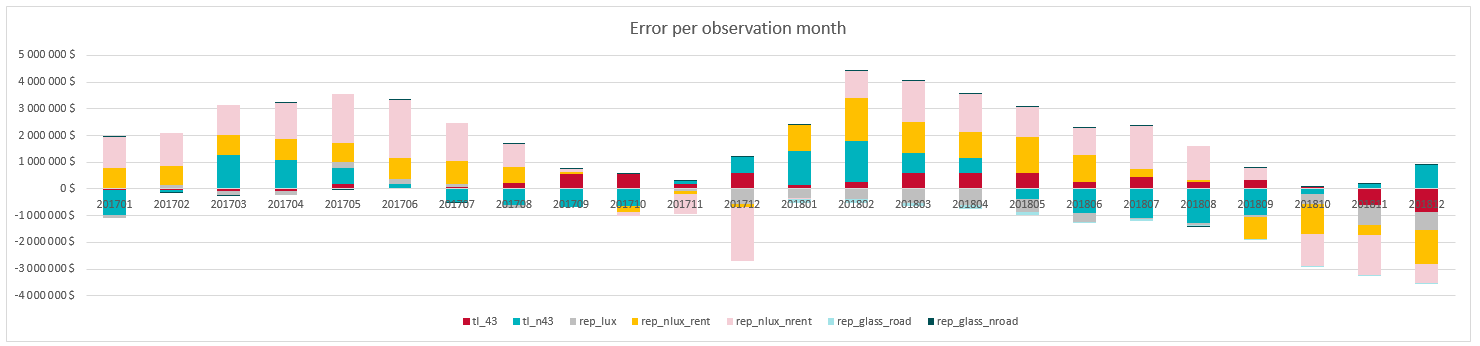
\includegraphics[scale=0.4]{Graphiques/QC_current_model_by_month} 
				\renewcommand{\figurename}{Figure}
				\caption{Quebec "Historical  pending claims" model, prediction error by observation month}\label{Fig_QC_current_er_by_month}
			\end{center}
		\end{figure}
		Figure \ref{Fig_QC_current_er_boxplot} indicates that the largest proportion of error comes form \texttt{tl\_n43} and \texttt{rep\_nlux\_nrent}.These two \texttt{leaf} are also the largest in terms of volume. 
		\begin{figure}[H]
			\begin{center}
				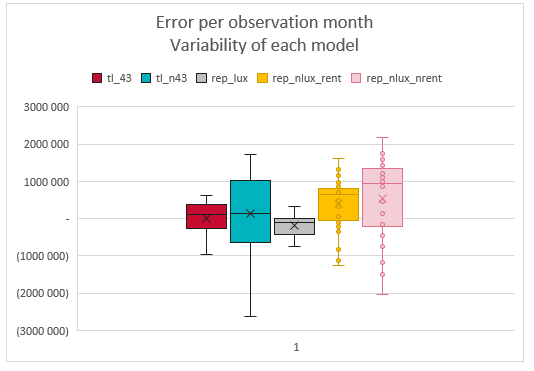
\includegraphics[scale=0.4]{Graphiques/QC_current_model_mustach} 
				\renewcommand{\figurename}{Figure}
				\caption{Quebec "Historical  pending claims" model, monthly prediction error boxplot}\label{Fig_QC_current_er_boxplot}
			\end{center}
		\end{figure}
	
	\paragraph{Ontario:}
		In Ontario, our model has the tendency to underestimate the ultimate amount. The average error per observation month shown in figure \ref{Fig_ON_current_er_by_month} is at -4632281.66. Specifically the winter proves difficult for our model. We are currently investigating this issue, but it might be related to the lag we use and/or the trends observed in the data.
		\begin{figure}[H]
			\begin{center}
				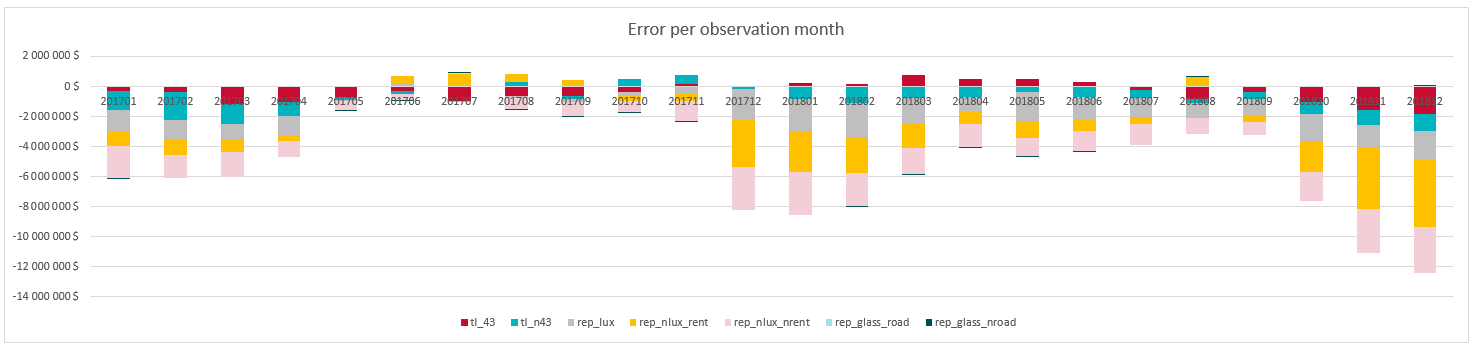
\includegraphics[scale=0.4]{Graphiques/ON_current_model_by_month} 
				\renewcommand{\figurename}{Figure}
				\caption{Ontario "Historical  pending claims" model, prediction error by observation month}\label{Fig_ON_current_er_by_month}
			\end{center}
		\end{figure}
		\begin{figure}[H]
			\begin{center}
				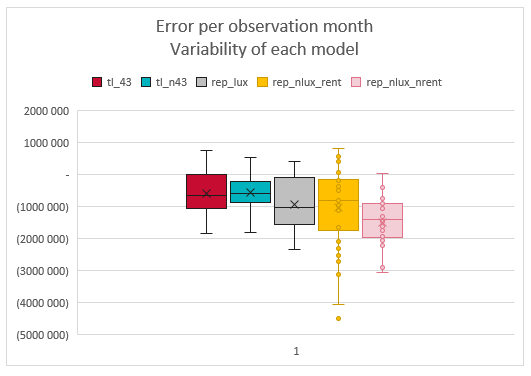
\includegraphics[scale=0.4]{Graphiques/ON_current_model_mustach} 
				\renewcommand{\figurename}{Figure}
				\caption{Ontario "Historical  pending claims" model, monthly prediction error boxplot}\label{Fig_ON_current_er_boxplot}
			\end{center}
		\end{figure}
	\paragraph{Alberta:}
		The average monthly prediction error amounts to 3547625.79 on a total volume of about 80 million. There is no clear seasonal pattern, however the model constantly overestimates. The cause of the overestimation is the subrogation, which even after 12 months is not completed. We found about 10\% of the claims in Alberta still receive recovery payments after 12 months. Figure \ref{Fig_AB_current_er_boxplot} shows that \texttt{rep\_nlux\_rent} is the biggest source of error for this model.   
		\begin{figure}[H]
			\begin{center}
				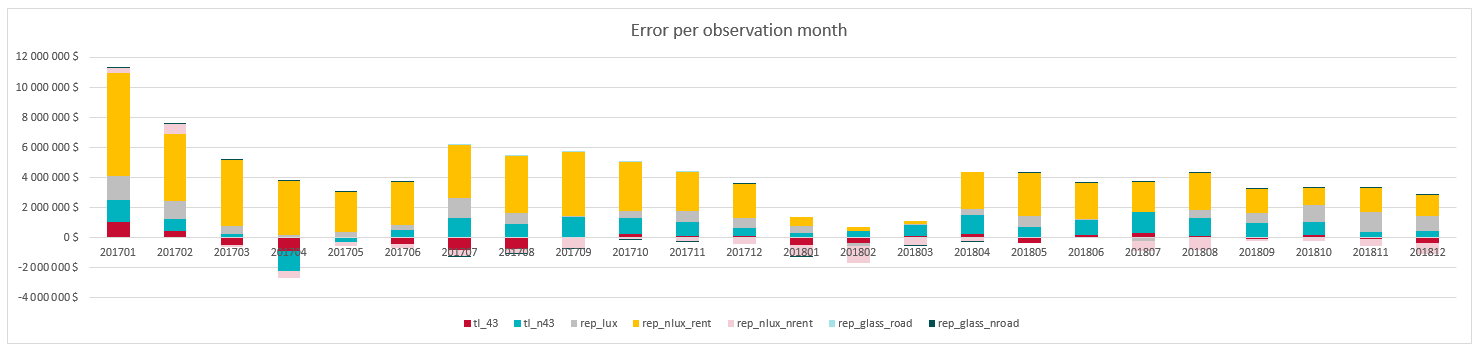
\includegraphics[scale=0.4]{Graphiques/AB_current_model_by_month} 
				\renewcommand{\figurename}{Figure}
				\caption{Alberta "Historical  pending claims" model, prediction error by observation month}\label{Fig_AB_current_er_by_month}
			\end{center}
		\end{figure}
		\begin{figure}[H]
			\begin{center}
				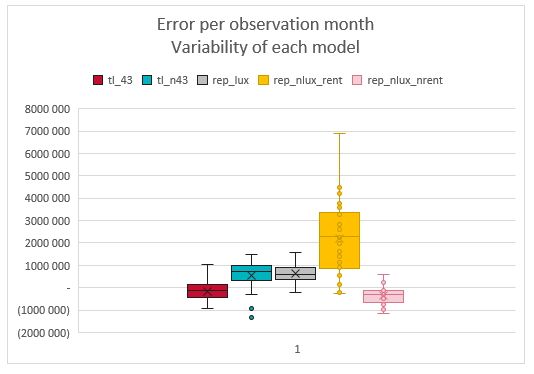
\includegraphics[scale=0.4]{Graphiques/AB_current_model_mustach} 
				\renewcommand{\figurename}{Figure}
				\caption{Alberta "Historical  pending claims" model, monthly prediction error boxplot}\label{Fig_AB_current_er_boxplot}
			\end{center}
		\end{figure}
	
\subsection{Second model iteration: Historical pending but now closed claims}
	Excluding open claims in the factor calculations has a strong impact on the model. The average monthly error are -1379997.20, -5134385.50 and -431987.83, for Quebec, Ontario and Alberta respectively. This model has a strong tendency to underestimate. Albeit, for Alberta, when looking at figure \ref{Fig_AB_closedonly_er_by_month}, the results are considerably better than the first iteration model. Adding open claims seems to multiply the error by a factor of 10. This indicated that once a claim is closed, the subrogation process seems to also be finished or partly finished. For the other two provinces, it that adding open claims captures something we are not yet able to fully explain. We suspect that the issue is related to the imputation method and observed trends.
		\begin{figure}[H]
			\begin{center}
				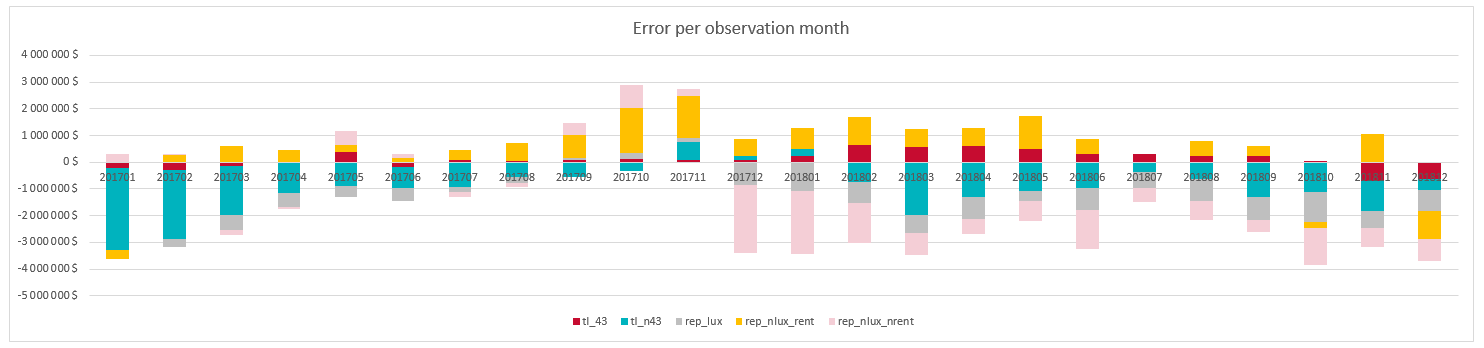
\includegraphics[scale=0.4]{Graphiques/QC_closedonly_model_by_month} 
				\renewcommand{\figurename}{Figure}
				\caption{Quebec "Historical  pending but now closed claims" model, prediction error by observation month}\label{Fig_QC_closedonly_er_by_month}
			\end{center}
		\end{figure}
		\begin{figure}[H]
			\begin{center}
				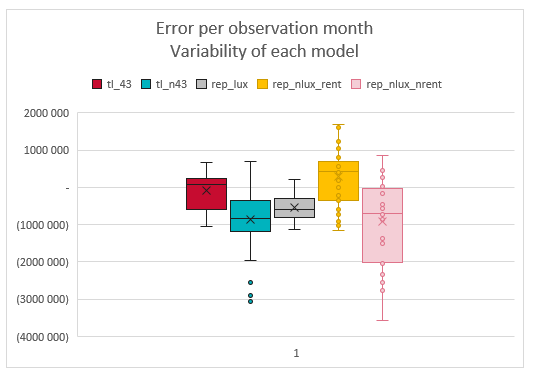
\includegraphics[scale=0.4]{Graphiques/QC_closedonly_model_mustach} 
				\renewcommand{\figurename}{Figure}
				\caption{Quebec "Historical  pending but now closed claims" model, monthly prediction error boxplot}\label{Fig_QC_closedonly_er_boxplot}
			\end{center}
		\end{figure}

		\begin{figure}[H]
			\begin{center}
				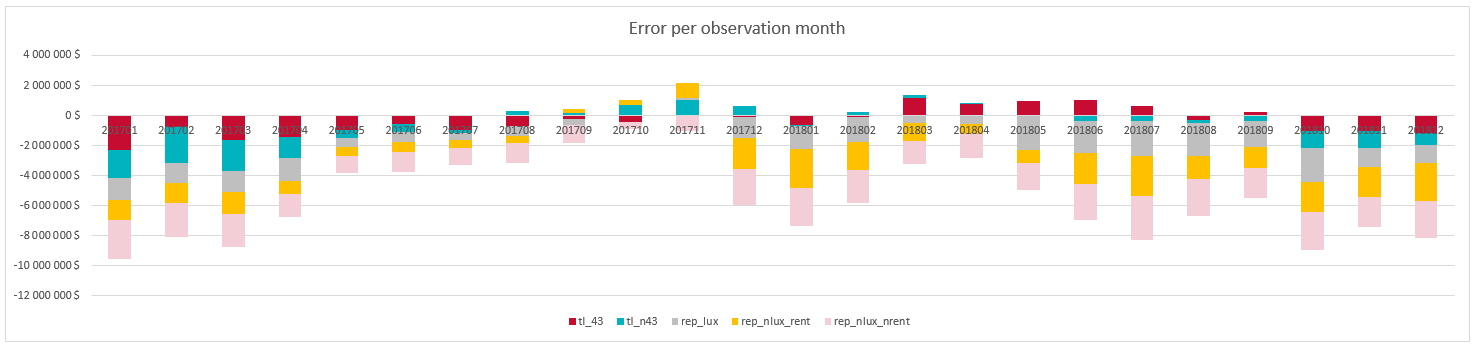
\includegraphics[scale=0.4]{Graphiques/ON_closedonly_model_by_month} 
				\renewcommand{\figurename}{Figure}
				\caption{Ontario "Historical  pending but now closed claims" model, prediction error by observation month}\label{Fig_ON_closedonly_er_by_month}
			\end{center}
		\end{figure}
		\begin{figure}[H]
			\begin{center}
				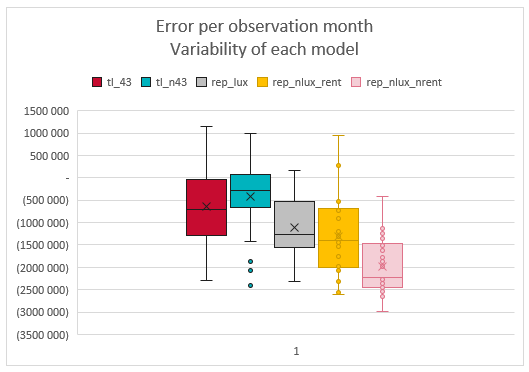
\includegraphics[scale=0.4]{Graphiques/ON_closedonly_model_mustach} 
				\renewcommand{\figurename}{Figure}
				\caption{Ontario "Historical  pending but now closed claims" model, monthly prediction error boxplot}\label{Fig_ON_closedonly_er_boxplot}
			\end{center}
		\end{figure}


		\begin{figure}[H]
			\begin{center}
				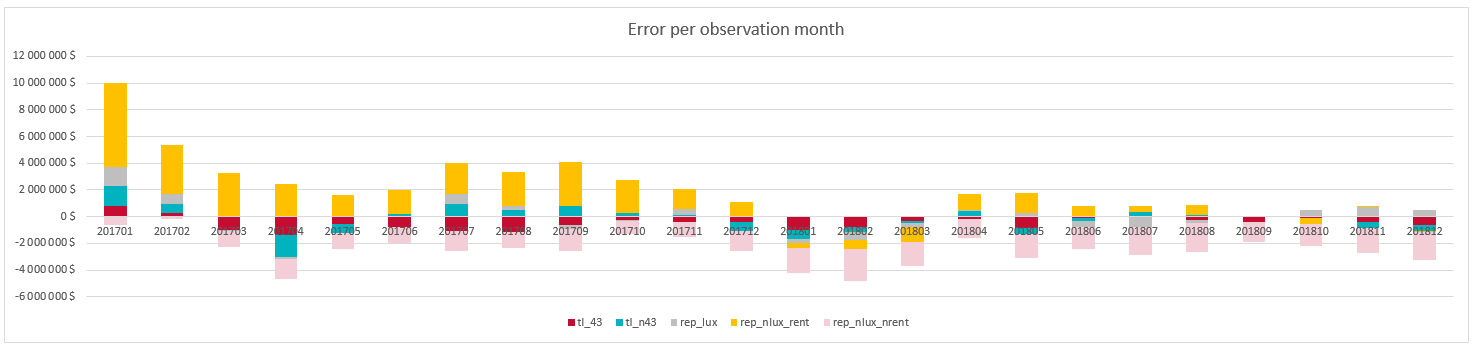
\includegraphics[scale=0.4]{Graphiques/AB_closedonly_model_by_month} 
				\renewcommand{\figurename}{Figure}
				\caption{Alberta "Historical  pending but now closed claims" model, prediction error by observation month}\label{Fig_AB_closedonly_er_by_month}
			\end{center}
		\end{figure}
		\begin{figure}[H]
			\begin{center}
				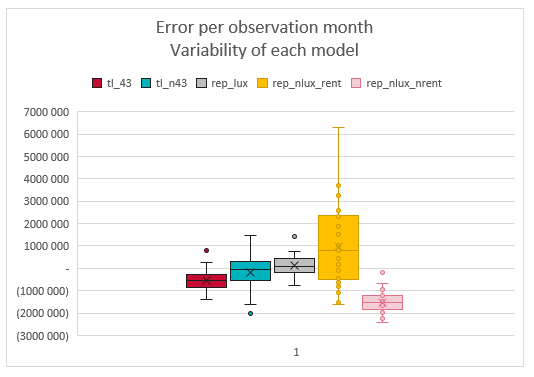
\includegraphics[scale=0.4]{Graphiques/AB_closedonly_model_mustach} 
				\renewcommand{\figurename}{Figure}
				\caption{Alberta "Historical  pending but now closed claims" model, monthly prediction error boxplot}\label{Fig_AB_closedonly_er_boxplot}
			\end{center}
		\end{figure}
	
\subsection{Third model iteration: Historical closed claims }
	Lastly, the third iteration model seems not to function as well as expected. Quebec has an average monthly error of -7196717.05, Ontario of -13153105.83 and Alberta of 4148104.04. One issue with this model is related to the claims in the window. While the two previous model use a small window of pending claims, this model uses all claims that closed in the time window. Thus, we are using claims that can be very old relative to the observation month. Therefore the age of a claim might have a considerable impact on this model.
	
	
		  
	\section{Conclusion}\label{Sect_Conclusion}
	bal bla	 
	
	\clearpage
	\bibliographystyle{apalike} % Bibliographie
	\bibliography{bibliographie}
	\clearpage
	
	\pagenumbering{arabic}% resets `page` counter to 1
	\renewcommand*{\thepage}{A\arabic{page}}
	\appendix

	
\end{document}